\documentclass[twoside,a4paper]{book}
\usepackage[ngerman]{babel}
\usepackage[utf8]{inputenc}
\usepackage[T1]{fontenc}
% \usepackage[top=2.5cm,bottom=1.75cm,right=2cm,left=2.3cm]{geometry}
\usepackage{lscape} % Seiten im Querformat
\usepackage{longtable}
% \usepackage{wrapfig}
\usepackage{shadethm}
\usepackage{color}
\usepackage{floatflt}
\usepackage{subfigure}
\usepackage{graphicx}
\usepackage{fancyhdr}
\usepackage{amsmath,amssymb}
\usepackage{nicefrac}
\usepackage{multicol}
\usepackage{enumerate}

% \setlength{\parindent}{0pt} %Absatz-Einr"uckung
% \setlength{\parskip}{12pt} %Absatz-Abst"ande


%%% Index %%%
\usepackage{makeidx}
\makeindex

%\usepackage{a4wide}



%%% Zeilenabstand %%%
% \usepackage{setspace} %Zeilenabstand bestimmbar in Dokumentenabschnitten
% oder:
% \linespread{$$Verh"altnis_zu_normalem_Zeilenabstand$$} %Wirkt global

%% Tabellen %%
\usepackage{booktabs}
\setlength{\tabcolsep}{5pt}
%Abst zw Spalten
\renewcommand{\arraystretch}{1.4}
%Vielfacher Spaltenabst zw Zeilen


%% Aufzaehlungen -- description %%
\usepackage{expdlist}




%Kopfzeile: \pagestyle{myheadings} %Kopfzeile hinzuf"ugen
%\markright{$$Kopfzeile$$} %Inhalt der Kopfzeile

%\pagestyle{fancy} %Genauer zu definierende Kopfzeile
%\fancyhead[OL,OC,OR,EL,EC,ER]{} %O: ungerade seiten, E: gerade Seiten,
%\fancyfoot[OL,OC,OR,EL,EC,ER]{} %L:Links, C:Mitte, R:Rechts (leere Klammer {} l"oscht)
%\renewcommand{\headrulewidth}{dicke} %Dicke der Linie oben
%\renewcommand{\footrulewidth}{dicke} %Dicke der Linie unten
%\addtolength{\headwidth}{l"ange} %Breite wird vergr"o"sert (ragt "uber Text raus)
%\addtolength{\headheight}{l"ange} %H"ohe wird vergr"o"sert

%\newtheorem{$$k"urzel$$}{$$Name im
%  Text$$} %Definiert eigene Umgebung (begin{k"urzel}...end)
\usepackage[colorlinks=true,linkcolor=black,citecolor=black,bookmarksnumbered=true,breaklinks=true,pdfstartview=FitH]{hyperref}
\hypersetup{pdftitle="ExPhys1Script", pdfauthor=Kopp}



%Eigene Komandos
\newcommand{\zitat}[1]{{\slshape \sffamily #1}}
         %hebt Zitate deutlich ab
\newcommand{\st}[1]{{\slshape \textbf #1}}
\newcommand{\diff}{\ensuremath{\, \mathrm{d}}}
\newcommand{\Ve}[1]{\ensuremath{\vec{#1}}}

\newcommand{\Mat}[1]{\ensuremath{\mathbf{#1}}}
\newcommand{\Ten}[1]{\ensuremath{{\mathcal{#1}}}}

\newcommand{\const}{\ensuremath{\text{\emph{const}}}}

\newcommand{\Folgt}{\ensuremath{~ \Rightarrow ~ ~ }}
\newcommand{\Impl}{\ensuremath{~ \Rightarrow ~ ~}}

\newcommand{\Laplace}{\ensuremath{\Delta \,}}
\newcommand{\Nabl}{\ensuremath{\Ve \nabla \,}}
\newcommand{\Rot}{\ensuremath{\Ve \nabla \times }}
\newcommand{\Grad}{\ensuremath{\Ve \nabla \,}}
\newcommand{\Div}{\ensuremath{\Ve \nabla \cdot }}




\newcommand{\e}{\ensuremath{\operatorname{e}}}
\newcommand{\E}{\ensuremath{\operatorname{e}}}
\newcommand{\I}{\ensuremath{\operatorname{i}}}



%% Besonderes
% Vektorpotential
\newcommand{\Apot}{\ensuremath{\mathcal{A}}}
\newcommand{\mdm}{\ensuremath{\mu}}
    % magnetisches Dipolmoment


%% Formatierung



%\newshadetheorem{Def}{Definition}[section]
\newshadetheorem{Wichtig}{Wichtig!}

\newshadetheorem{Defi}{Definition}[chapter]
\newenvironment{Def}[1][]{%
\definecolor{shadethmcolor}{rgb}{.95,.95,.95}%
\definecolor{shaderulecolor}{rgb}{0.8,0.8,0.8}%
\setlength{\shadeboxrule}{1pt}%
\begin{Defi}[#1]%
 }{\end{Defi}}


\newenvironment*{Beispiel}[0]{$\diamondsuit$\sffamily}{ \hfill $\diamondsuit$}

\newcommand{\abs}[0]{\bigskip \noindent}

\newenvironment*{Einschub}[0]{$\rightarrow$ \indent}{$\leftarrow$}

\usepackage{units}




\setcounter{secnumdepth}{4} %Paragraph wird nummeriert
%\def\theparagraph{\textit{\mdseries\underline{\roman{paragraph}.}}}

\def\theparagraph{$\rhd$ (\alph{paragraph})} 
%Paragraph bekommt statt nummer ein Dreieck

%\def\theparagraph{$\rhd$ (\arabic{subsubsection} \alph{paragraph})}


% \usepackage{sectsty}
% \paragraphfont{\sffamily}

%\def\thefigure{\arabic{section}.\arabic{figure}\textsuperscript{\arabic{page}}}
%\def\theequation{\arabic{section}.\arabic{equation}\textsuperscript{\arabic{page}}}



%% Captions %%
\usepackage[format=hang,labelfont={bf,it},textfont=sl]{caption}



%% Referenzen %%
%\usepackage[german]{varioref}
% mit \vref{label} wird eine individuelle
% Bezeichnung verwendet; je nach dem,
% wie weit label und vref auseinander liegen.






%%%%%%%%%%%%%%%%%%%%%%%%%%%%%%%%%%%%%%%%%%%%%%%%%%%%%%%%%%%%

%%%%%%%%%%%%%%%%%%%%%%%%%%%%%%%%%%%%%%%%%%%%%%%%%%%%%%%%%%%%

%%%%%%%%%%%%%%%%%%%%%%%%%%%%%%%%%%%%%%%%%%%%%%%%%%%%%%%%%%%%
 
\title{Experimentalphysik III}

\author{Michael Kopp}

\date{Version $\alpha ~ 0.1$ ~ --- ~ \today}





% \begin{titlepage}
%    \author{Michael Kopp}
% \title{Experimentalphysik I}
% \end{titlepage}




%%%%%%%%%%%%%%%%%%%%%%%%%%%%%%%%%%%%%%%%%%%%%%%%%%%%%%%%%%%%

%%%%%%%%%%%%%%%%%%%%%%%%%%%%%%%%%%%%%%%%%%%%%%%%%%%%%%%%%%%%

%%%%%%%%%%%%%%%%%%%%%%%%%%%%%%%%%%%%%%%%%%%%%%%%%%%%%%%%%%%%


\begin{document}


\frontmatter

%\maketitle

\begin{titlepage}
\begin{center}
\vspace{3em}

{\large \sc  Michael Kopp}\\[8em]
~ ~ 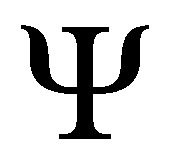
\includegraphics[width=0.45\textwidth]{psi}\\[5em]
{\huge \bf Script}\\[0.03\textheight]
{zur Vorlesung}\\[0.08\textheight]
%{\fontfamily{phv}\fontsize{50px}{1px} \selectfont Experimentalphysik
%I}\\
\hrule ~\\[0.4cm]
{\bf \fontsize{35px}{1px} \selectfont Experimentalphysik III}\\[0.4cm]
\hrule ~ \\[8em] %12
{bei Prof. M. Dressel, Uni Stuttgart, 2010}

\vfill

{ \today \\(Version $\alpha$ 0.1)}
\end{center}
\end{titlepage}


\addcontentsline{toc}{chapter}{Inhaltsverzeichnis}
\tableofcontents


\sloppy		
           % Macht keine BadBoxes

%Zeilenabstand:
%Wenn "`setspace"' aktiviert:
	%\singlespacing
	%\onehalfspacing
	%\doublespacing

%\setlength{\parskip}{8pt}
%\setlength{\parindent}{0pt}






% \setcounter{chapter}{-1}


\chapter{Vorwort}
\label{kap_vorwort}

Mal sehen, wie lange ich es dieses Semester durchhalte ;-)

\vfill
\hfill \textit{Michael Kopp}

\hfill Besigheim, \today





\mainmatter

%%%%%%%%%%%%%%%%%%%%%%%%%%%%%%%%%%%%%%%%%%%%%%%%%%%%%%%%%%%%%%
%%%%%%%%%%%%%%%%%%%%%%%%%%%%%%%%%%%%%%%%%%%%%%%%%%%%%%%%%%%%%%
%%%%%%%%%%%%%%%%%%%%%%%%%%%%%%%%%%%%%%%%%%%%%%%%%%%%%%%%%%%%%%
%%%%%%%%%%%%%%%%%%%%%%%%%%%%%%%%%%%%%%%%%%%%%%%%%%%%%%%%%%%%%%
%%%%%%%%%%%%%%%%%%%%%%%%%%%%%%%%%%%%%%%%%%%%%%%%%%%%%%%%%%%%%%










\chapter{EM-wellen?}
\label{kap_em-wellen}


\section{Maxwell-Gleichungen}
\label{kap_maxwell-gleichungen}



\subsection{Wellengleichung}
\label{kap_wellengleichung}




In \textbf{Materie} gelten die vier Maxwell-Gleichungen:
\begin{Wichtig}[Maxwell-Gleichungen in Materie]
   \begin{eqnarray}
      \label{eq:1}
      \Rot \vec E + \frac{\partial }{\partial t} \vec B = \vec 0 & \text{Induktion} \\
      \label{eq:2}
      \Div \vec B = 0 & \text{keine magn. Monopole}\\
      \label{eq:3}
      \Rot \vec H - \frac{\partial }{\partial t}\vec D = \vec j &
      \text{el. Feld od. Strom erz. magn. Feld}\\
      \label{eq:4}
      \Div \vec D = \varrho & \text{Lad. erz. el. Feld}
   \end{eqnarray}
\end{Wichtig}

Es gelten die Zusammenh"ange
\begin{Wichtig}
   [El. und Magn. Feld in Materie\index{Felder in Materie}]
\begin{eqnarray}
   \label{eq:7}
   \vec D &=& \varepsilon_0 \cdot \varepsilon \cdot \vec E  ~ \text{ und
   }\\
   \label{eq:8}
   \vec B &=& \mu_0 \cdot \mu \cdot \vec H \;.
\end{eqnarray}
\end{Wichtig}


Wir wollen im Folgenden die \st{Vereinbarung} treffen, dass wir
\emph{nicht-magnetische} Meterialien annehmen. Au"serdem sollen keine
Str"ome oder Ladungen vorliegen; also
\begin{equation}
   \label{eq:6}
   \mu = 1, ~ \vec j = \vec 0 \text{ und } \varrho = 0 \;.
\end{equation}
Allerdings k"onnen wir nicht $\varepsilon=0$ setzen.


\begin{Einschub}
Die \st{Permittivit"at $\varepsilon$} ist in \textbf{\index{anisotrope
    Materialien}anisotropen Materialien} kein Skalar mehr, sonder ein
Tensor $\Ten \varepsilon$. Dar"uber hinaus muss $\Ten \varepsilon$
nicht mal linear sein, sondern kann auch
\begin{equation*}
   \varepsilon = \Ten \varepsilon = \Ten \varepsilon(\vec E)
\end{equation*}
sein. In Gasen ist normalerweise $\varepsilon \approx 1$ und in Gasen,
Fl"ussigkeiten und kubischen (also sehr symmetrischen) Kristallen ist
$\varepsilon$ skalar. Die "ubrigen, nicht inearen F"alle von
$\varepsilon$ f"uhren zu interessanten Effekten, die in der
sog. \emph{\index{Nichtlinearen Optik}Nichtlinearen Optik} behandelt
werden.   
\end{Einschub}


Mit den oben genannten Vereinfachungen erhalten wir als neue
"`Arbeitsgrundlage"' die Maxwellgleichungen:
\begin{eqnarray}
   \label{eq:9}
   \Rot \vec E &=& - \frac{\partial }{\partial t}\vec B \;,\\
\label{eq:5}
\Div \vec E &=& 0 \;,\\
\label{eq:10}
\Rot \vec B &=& \mu_0 \frac{\partial }{\partial t}\vec D \;,\\
\label{eq:11}
\Div \vec B &=& 0 \;.
\end{eqnarray}

Wenden wir nun $\Rot$ auf \eqref{eq:9} an, erhalten wir f"ur die linke Seite
\begin{eqnarray*}
   \Rot (\Rot \vec E) = \Grad (\Div\vec E) - \Laplace \vec E = - \Laplace
   \vec E
\end{eqnarray*}
und f"ur die rechte
\begin{eqnarray*}
   \Rot (-\frac{\partial }{\partial t}\vec B) = -\frac{\partial
   }{\partial t}\Rot \vec B 
\stackrel{\eqref{eq:10}}{=}
- \mu_0 \frac{\partial^2}{\partial t^2} \vec D
\stackrel{~\eqref{eq:7}}{=}
- \mu_0 \frac{\partial^2}{\partial t^2} \varepsilon_0 \varepsilon \,
\vec E \;.
\end{eqnarray*}
Es gilt also
\begin{equation}
   \label{eqn_wellengl_e}
 \boxed{\Laplace \vec E = \mu_0  \varepsilon_0 \varepsilon
   \frac{\partial^2}{\partial t^2} \, \vec E \;. }
\end{equation}
Analog kommt man auch auf
\begin{equation}
   \label{eqn_wellengl_b}
 \boxed{\Laplace \vec B = \mu_0  \varepsilon_0 \varepsilon
   \frac{\partial^2}{\partial t^2} \, \vec B \;. }
\end{equation}
\begin{Wichtig}
   Diese beiden Gl. sind
   \emph{\index{Wellengleichungen}Wellengleichungen} der
   Elektromagnetischen Welle.
\end{Wichtig}

\begin{Einschub}
   Wir werden sehen, dass
   \begin{equation}
      \label{eq:14}
      v_{ph} = \frac{1}{\sqrt{\varepsilon \, \varepsilon_0\,
          \mu_0}} = \frac{c_0}{\sqrt{\varepsilon}} =: \frac{c_0}{n}
   \end{equation}
   gilt. Im Vakuum ist mit $\varepsilon =1$ $v_{ph} = c_0$; damit
   sieht man auch, dass $\varepsilon \leq 1$ sein muss, da sich sonst
   Informationen schneller als $c_0$ ausbreiten k"onnten...
\end{Einschub}
\begin{Def}
   [\index{Brechungsindex}Brechungsindex $n$]
   Der Brechungsindex kennzeichnet die Brechung, also die
   Richtungs"anderung von Elektromagnetischen Wellen beim "Ubergang
   zwischen zwei Medien. Es gilt
   \begin{equation}
      \label{eqn_def_n}
      n = \sqrt{\varepsilon} = \frac{c_0}{c} \;.
   \end{equation}
\end{Def}


Wir suchen nun \st{L"osungen f"ur die Wellengleichungen}. 
Eine Einfache L"osung ist eine \textbf{ebene Welle}:
\begin{equation}
   \label{eq:16}
   \vec E = \vec E(\vec r,t) = \vec E_0 \cdot \exp \left (\I (\omega t -
   \vec k \vec r + \varphi ) \right ) \;,
\end{equation}
wobei wir mit $\vec k$ den \emph{\index{Wellenvektor}Wellenvektor}
bezeichnen. Er zeigt in Richtung der Ausbreitung und hat den Betrag
\begin{equation}
   \label{eqn_def_k}
   \|\vec k \| = k = \frac{2\pi}{\lambda} \, n \;.
\end{equation}
Dabei brauchen wir das $n$ hier, weil wir mit $\lambda$ die
\index{Vakuumwellenl"ange}Vakuumwellenl"ange meinen. In einem Medium
mit $n \neq 1$ ver"andert sich die Wellenl"ange logischerweise. Das
$n$ kann dabei $n = n(\omega)$ sein.

$\vec k$ ist die r"aumliche Entsprechung von $\omega$: Bewegt man sich
um $\lambda/n$ weiter, so hat die Welle wieder den gleichen
Phasenzustand. Dies "au"sert sich darin, dass das Argument des $\exp$
aus \eqref{eq:16} sich um $2\pi$ ge"andert hat.

\begin{Wichtig}
   [\index{Dispersionsrelation}Dispersionsrelation]
Die D. ist allgemein ein Zusammenhang zwischen Wellenzahl $k$ und
Kreisfrequenz $\omega$. In der Optik gilt:
\begin{equation}
   \label{eqn_dispersionslreation}
   \boxed{k = \frac{n \, \omega}{c} } \;.
\end{equation}
\end{Wichtig}
Die Herleitung dieser Formel ist einfach: Man setzt die Definition von
$\vec k$ \eqref{eqn_def_k} und die Definition von $\omega$ ($\omega =
2\pi\, \nu$) ein, und erh"alt
\begin{equation*}
   \frac{2\pi}{\lambda} \, n = n \, \frac{2\pi \, \nu}{c} \text{
     also }
\lambda \, \nu = c \;;
\end{equation*}
dies entspricht $s/t = v$.


\begin{Einschub}
   Auch wenn Gl. \eqref{eq:16} die Wellengleichung
   \eqref{eqn_wellengl_e} l"ost, so wird sie in der Natur doch nie
   betrachtet werden k"onen, weil die Natur keine komplexen Zahlen
   kennt. Wir m"ussen also entweder den Real- oder Imagin"arteil von
   \eqref{eq:16} verwenden, oder wir addieren
   \begin{equation*}
      2\, \vec E' = \vec E + \bar{\vec E}\;,
   \end{equation*}
   wobei $\bar{\vec E}$ das komplex konjugierte von $\vec E$ ist.
\end{Einschub}

Wendet man auf \eqref{eq:16} $\Div$ an, so findet man mit den Maxwellgl.
\begin{equation*}
   \Div \Vec E = - \I \, \vec k \cdot \vec E \stackrel{~\eqref{eq:5}}{=} 0 \;.
\end{equation*}
\begin{Einschub}
   Dies findet man aber nur bei unseren Vereinfachungen; im
   Allgemeinen ist nur $\vec D$ senkrecht zu $\vec k$. Erst wenn die
   Materie, die die Welle durchl"auft isotrop ist, ist die
   Elektromag. Welle eine Transversalwelle.
\end{Einschub}

Wenn wir die Wellengleichung f"ur das magnetische Feld ebenso l"osen
(also analog zu \eqref{eq:16}, finden wir auch, dass 
\begin{equation*}
   \vec B \perp \vec k
\end{equation*}
ist. 
\begin{Wichtig}
   Elektrisches und Magnetisches Feld stehen senkrecht zur
   Ausbreitungsrichtung.
\end{Wichtig}
Betrachtet man nun oBdA\footnote{Wir haben hier eine lineare Theorie
  vor uns. Damit kann man eine L"osung als endliche Summe einfacherer
  L"osungen betrachten...} $\vec E_0 = (A,0,0)^T$ und $\vec k = (0, 0, k)$, dann erh"alt man als
Rotation:
\begin{equation*}
   \Rot \vec E =  (0, -\I \, k, 0)^T \, \vec E
   \stackrel{~\eqref{eq:9}}{=} - \frac{\partial }{\partial t}\vec B \;.
\end{equation*}
Dies kann man einfach hochintegrieren: Man erh"alt:
\begin{equation}
   \label{eq:12}
   \vec B = \vec B(\vec r,t) = (0, -\frac{k}{\omega}, 0)^T \, \vec E
\end{equation}
So sieht man leicht:
\begin{Wichtig}
   Magnetisches und Elektrisches Feld sind senkrecht zueinander.
\end{Wichtig}
Man findet statt \eqref{eq:12} den Zusammenhang
\begin{equation}
   \label{eqn_zsht_b-e}
   \boxed{ \vec B = \frac{1}{\omega} \, \left ( \vec k \times \vec E
     \right ) } \;,
\end{equation}
wenn mam mit allgemeinen Gr"o"sen bei der Herleitung arbeitet.

Damit gilt f"ur die Amplituden der Zusammenhang
\begin{equation}
   \label{eq:13}
   B = \frac{k}{\omega} \, E \text{ oder mit
     \eqref{eqn_dispersionslreation}: } 
B = \frac{n}{c} \, E \;.
\end{equation}
\begin{Einschub}
   In Gau"seinheiten gilt elegant:
   \begin{equation*}
      E = B \;.
   \end{equation*}
\end{Einschub}


\abs
Uns bleibt, wenn wir die Ausbreitungsrichtung der Welle kennen, noch
ein Freiheitsgrad f"ur ihre Orientierung: Dies ist die
\textbf{Polarisation}. Sie gibt an, in welche Ebene die E-Komponente
der Welle geneigt ist. Sie kann in jede beliebige Richtung zeigen und
diese Richtung kann von Zeit und Ort abh"angen.\footnote{Weil es sich
  um einen unbestimmten \emph{Freiheits}grad handelt.}

\abs
Die Wellen decken einen gro"sen \textbf{Frequenzbereich} ab. Wir k"onnen nur
einen kleinen davon sehen; zwischen Ultraviolett mit ca \unit[400]{nm}
und Infrarot mit \unit[800]{nm}. Beim Sehen ist die Aufl"osung durch
die Wellenl"ange beschr"ankt: Letztere muss kleiner sein als der
minimale Abstand zwischen zwei zu beobachtenden Punkten. Kleinere
Wellenl"angen f"ur mehr Details gehen mit gr"o"seren Energien einher.








\subsection{Energie und Impuls von EM-Wellen}
\label{kap_energie-und-impuls-von-em}

Sonnenlicht is \emph{warm}. Folglich m"ussen EM-Wellen Energie
"ubertragen k"onnen. Wir definieren asl Ma"se daf"ur:
\begin{Def}
   [\index{Energiestrahldichte}Energiestrahldichte $\vec S$]
   \begin{equation}
      \label{eqn_def_energiestrahldichte}
      \vec S = \vec E \times \vec H \;.
   \end{equation}
Sie gibt uns die "ubertragene Energie pro Fl"che an.
\end{Def}
Mit der Einheit $[S] = \unitfrac[1]{W}{m^2}$. Durch unsere Vereinbarungen gilt f"ur uns:
\begin{equation}
   \label{eq:17}
         \vec S = \vec S(\vec r,t) = \frac{1}{\mu_0} \, \left ( \vec E
         \times \vec B \right ) = \varepsilon_0 \, c_0^2 \, \left (
         \vec E \times \vec B \right ) \;.
\end{equation}
$\vec S$ zeigt also \emph{in isotropen Medien} in Ausbreitungsrichtung (weil $\vec k \perp \vec
E$ und $\vec k \perp \vec B$).

Weil aber $\vec E$ und $\vec B$ nicht konstant sind, verwenden wir
noch eine zeitunabh"angige Definition:
\begin{Def}
   [\index{Lichtintensit"at}Lichtintensit"at $I$]
Auch \emph{\index{Energiestromdichte}Energiestromdichte} genannt:

Die im (zeitlichen) Mittel auf eine Einheitsfl"ache senkrecht zu $\vec
k$ transportierte Energie:
   \begin{equation}
      \label{eqn_def_lichtintensitaet}
      I = \langle \, \| \vec S \| \,  \rangle
      \stackrel{~\eqref{eq:13}}{=}
\varepsilon_0 \, n\, c_0 \cdot \langle \, \| \vec E \|^2  \rangle
   \end{equation}
\end{Def}
F"ur eine Ebene Welle gilt wegen $\langle \cos^2  \rangle =
\frac{1}{2}$:
\begin{equation*}
   I^\text{Ebene Welle} = \frac{1}{2} \, \varepsilon_0 \, n\, c_0
   \cdot \| \vec E_0 \|^2\;.
\end{equation*}


Um den Impuls einer Welle sinnvoll definieren zu k"onnen, brauchen wir
noch:
\begin{Def}
   [\index{Strahlungsdruck}Strahlungsdruck $P_s$]
auch \emph{\index{Lichtdruck}Lichtdruck} genannt: 

Die Kraft, die elektroagnetische Strahlung pro Fl"ache auf ein
Material aus"ubt.
\end{Def}
Anschaulich wird dies, wenn man den Teilchencharacter des Lichts
bedenkt: Ein Photon hat Masse und Geschwindigkeit und damit auch einen
Impuls $p = \frac{h}{\lambda}$, den es an einen K"orper "ubertragen
kann. Reflektiert der K"orper total, so wird der doppelte Impuls
"ubertragen, als wenn er vollst"andig absorbiert: Die Photonen haben
im ersten Fall nach dem "`Sto"s"' den Impuls $-p$ und konnten so
$p-(-p) = 2p$ "ubertragen. In letzterem Fall haben sie nach dem Sto"s
$p=0$.

Es gilt der Zusammenhang
\begin{equation}
   \label{eq:15}
   P_s^\text{absorbiert} = \frac{I}{c} \text{ und }
P_s^\text{total reflektiert} = 2 \frac{I}{c}\;.
\end{equation}
\begin{Beispiel}
   Sonnenlicht hat $I \approx \unitfrac[1,5]{W}{m^2}$ und damit einen
   Strahlungsdruck von $P_s \approx \unit[5 \cdot 10^{-6}]{Pa}$.
\end{Beispiel}








\subsection{Fourier}
\label{kap_fourier}


Weil wir -- wie bereits oben erw"ahnt -- mit einer linearen Theorie
arbeiten, k"onnen wir Wellen (L"osungen von DGL) linearkombinieren um
weitere Wellen (L"osungen) zu erhalten. Ein m"achtiges Werkzeug stellt
daf"ur \textsc{\index{Fourier}Fourier} zur Verf"ugung. Man kann damit
eine gro"se Klasse von Wellen als Linearkombination
bzw. Integral\footnote{In diese Sinne ist ein Integral nur die
  konsequente Fortsetzung einer Summe/Reihe; Man h"atte (\ref{eq:18})
  auch als Reihe schreiben k"onnen durch $\sum_{\omega = -
    \infty}^{+\infty} = \frac{1}{2\pi} \int_{-\infty}^{+\infty}$.}
darstellen:
\begin{equation}
   \label{eq:18}
   \vec E(\vec r,t) 
= 
\frac{1}{2\pi} \int_{- \infty}^{+ \infty} 
\underbrace{ \int_{-\infty}^{+\infty} \vec E(\vec r,t) \, \E^{- \I
    \, \omega \, t} \diff t }_{\vec E(\vec r,\omega)} \, \E^{\I \, \omega \, t}
\diff \omega \;.
\end{equation}
Hier ist schon angedeutet, dass man durch die Fourieranalyse aus einer
Funktion $\vec E : (\vec r,t) \mapsto \vec E(\vec r,t)$ im Zeit-Raum
eine Funktion $\vec E : (\vec r,\omega) \mapsto \vec E(\vec r,\omega)$
im Frequenz-Raum machen kann -- analog k"onnte man genausogut den
$k$-Raum betrachten -- dann w"urde aus $\vec E : (\vec r,t) \mapsto
\vec E(\vec r,t)$ eine Funktion $\vec E : (\vec k,t) \mapsto \vec
E(\vec k,t)$. Die Betrachtung in diesen R"aumen macht dann Sinn, wenn
man es mit periodischen -- zeitlichen wie
r"aumlichen\footnote{Beispielsweise ein Kristall: Bei Kristallanalysen
  rechnet man in $k$-R"aumen.} -- Vorg"angen zu tun hat.


\begin{Beispiel}
   \st{Fouriertransformation} einer \textsc{Gauss}-Kurve. Eine
   Gauss-Kurve im Frequenzenraum ist definiert "uber
   \begin{equation*}
      E(\omega) = A \cdot \exp \left ( - \left ( \frac{\omega -
              \omega_0}{\delta_\omega} \right )^2 \right ) \;.
   \end{equation*}
   Dabei gibt $\delta_\omega$ die halbe Breite (Abstand Mitte--Rand) an, die die Kurve in
   der H"ohe $E = A/\E$ hat. $A$ ist die maximale H"ohe der Kurve und
   $\omega_0$ gibt den "`$x$"'-Wert an, bei dem sich das
   Max. befindet.

   Die Fouriertransformation ist dann:
   % \begin{eqnarray*}
%       E(t) &=& \frac{1}{2\pi} \, \int_{-\infty}^{+\infty} E(\omega) \, \E^{\I \omega t}
%       \diff \omega 
%       = 
%       \frac{1}{2\pi} \, \int_{-\infty}^{+\infty} A \cdot \E^{ - \left ( \frac{\omega -
%              \omega_0}{\delta_\omega} \right )^2 } \, \E^{\I \omega t}
%       \diff \omega\\
%       &=& 
% \frac{1}{2\pi} \, \int_{-\infty}^{+\infty} A \cdot \E^{ - \left ( \frac{\omega -
%              \omega_0}{\delta_\omega} \right )^2 + \I \omega t } 
%       \diff \omega\\
% &\stackrel{\ast}{=}&
% \frac{1}{2\pi} \, \int_{-\infty}^{+\infty} A \cdot \E^{ \overbrace{-\frac{1}{\delta_\omega^2} \left (
%      \omega + \frac{\I t \delta_\omega^2 + 2 \omega_0}{2} \right
%   )^2}^{- r^2}
%   + \overbrace{\left ( \frac{\I t \delta_\omega^2 + 2 \omega_0}{2} \right )^2 -
%   \frac{\omega_0^2}{\delta_\omega^2} }^\text{nicht von $\omega$ abh.}}
% \diff r\\
% &=&
% \frac{1}{2\pi} \, A \, \sqrt{\pi} \cdot \E^{\left ( \frac{\I t \delta_\omega^2 + 2 \omega_0}{2} \right )^2 -
%   \frac{\omega_0^2}{\delta_\omega^2} }
% =
% \frac{1}{2 \, \sqrt{\pi}} \, A \, \E ^{(\omega_0 -
%   \frac{\omega_0^2}{\delta_\omega^2} - t^2 \frac{\delta_\omega^2}{4}) +
%   \I \,( \omega_0 t \delta_\omega^2)}
%    \end{eqnarray*}
   \begin{equation*}
      E(t) = \frac{A \, \delta_\omega}{2 \, \sqrt{\pi}} \, \E^{\I \,
        \omega_0 \, t} \cdot \E^{-\frac{\delta_\omega^2}{4} \, t^2}
   \end{equation*}
   Transformiert man diese Funktion wieder zur"uck, erh"alt man die
   Ausgangsfunktion. 
\end{Beispiel}
Hier sieht man durch Koeffizientenvergleich, dass 
\begin{equation}
   \label{eq:21}
   \frac{\delta_\omega^2}{2} = \frac{1}{\delta_t^2} \text{ oder }
   \delta_\omega \cdot \delta_t = 2 \;.
\end{equation}

   Damit hat man einen Zusammenhang zwischen den Breiten der
   Gauss-Kurven im $t$- und im $\omega$-Raum. Dies bedeutet aber noch
   mehr. Interpretiert man die Kurve als "`Streuung"' von Messwerten,
   kann man diese Gl. gewisserma"sen als
   \emph{\index{Unsch"arferelation}Unsch"arferelation} lesen; Um die
   Frequenz genau bestimmen zu k"onnen -- also $\delta_\omega$ klein
   zu machen -- braucht man gro"se $\delta_t$ -- also lange Messungen.


\begin{Beispiel}
Ein anderes Beispiel (zum \st{Hand-Rechnen}) ist mit $f(t) = \E^{-a \, t^2}$;
daf"ur gilt n"amlich:
\begin{eqnarray*}
   \hat f(\omega) &=& \int_{- \infty}^{+ \infty} f(t) \, \E^{-\I
     \omega t} \diff t 
= 
\int_{- \infty}^{+ \infty} \E^{-a \, t^2} \, \E^{-\I
     \omega t} \diff t\\
&=&
\int_{- \infty}^{+ \infty} \E^{-a (t^2 +\frac{\I \omega t}{a})} \diff
t\\
&\stackrel{\ast}{=}&
\int_{- \infty}^{+ \infty} \E^{-a (t + \frac{\I \omega}{a})^2 -
  \frac{\omega^2}{4 \, a}} \diff t\\
&=&
\sqrt{\pi / a} \, \E^{ - \frac{\omega^2}{4 \, a}}
\end{eqnarray*}
Hier sieht man sch"on, worauf es ankommt: Bei $(\ast)$ wird das
Argument von $\exp$ quadratisch erg"anzt und darunter wird das
bestimmte, uneigentliche Integral von $\E^{-r^2}$ gel"ost, wobei ein
Faktor "ubrig bleibt, der die neue Variable $\omega$ negativ
quadratisch enth"alt.
\end{Beispiel}

Hier sieht man, dass der Parameter $a$, der die Breite der Kurve
angibt, vorher mit $t^2$ multipliziert wurde, wobei jetzt dadurch
geteilt wird. D.h. eine dicke Gauss-Kurve geht durch
Fouriertransformation in eine d"unne "uber.




\subsection{Gruppen- und Phasengeschwindigkeit}
\label{kap_gruppen-und-phasengeschwindigkeit}



Wir wollen zuerst den Unterschied zwischen Gruppen- und
Phasengeschwindigkeit hervorheben. Dazu braucht man die Def.:
\begin{Def}
   [\index{Wellenpaket}Wellenpaket]
   Dies ist ein r"aumlich begrenzter Bereich auf einem Wellenleiter,
   auf dem sich eine (merklich von $0$ verschiedene) Amplitude
   zeigt. Dieser Bereich ist nicht fest, sonder wandert. Er kann dabei
   seine Breite ver"andern.
\end{Def}
Damit sich solch ein Wellenpaket bilden kann, m"ussen sich merere
(Elementar)Wellen aufaddieren; wie wir im Vorangegangenen Kapitel
gesehen haben, l"asst sich das durch eine Fourierreihe
bewerkstelligen.


Verwendet man eine Welle, die mit einer Gauss-Kurve moduliert ist,
spricht man von einem \emph{\index{Gaussschen Wellenpaket}Gaussschen
  Wellenpaket}; dabei multipliziert man eine Welle (bspw. Sinus) mit
der Gauss-Kurve und erh"alt so eine Kurve, die die Gauss-Kurve als
\emph{Einh"ullende} hat. Der gro"se Vorteil von einem solchen
Wellenpaket ist, dass nach Fouriertransformation die
Frequenzverteilung wieder eine Gauss-Kurven-Einh"ullende hat.

Wir wollen eine solche Welle verwenden. Die Funktion $E(\omega)$
ordnet jeder Frequenz eine geeignete Amplitude zu -- damit kann man
steuern, welche Elementarwellen in der "Uberlagerung wie stark
gewichtet werden sollen. Die Welle sieht also aus wie folgt:
\begin{equation}
   \label{eq:19}
   E(z,t) = \frac{1}{2\pi} \int_{- \infty}^{+ \infty} E(\omega) \cdot
   \underbrace{ \exp \, \I \left ( \omega \, t - k \, z  \right )
   }_\text{Elementarwelle} \diff \omega \;.
\end{equation}

Wir kennen aus (\ref{eqn_dispersionslreation}) die
\emph{Dispersionsrelation}, welche $k(\omega)$ beschreibt. Wir wollen
dieses $k$ nun in $\omega$ um $\omega_0$ entwickeln (mit neuer Variable
$\Omega$, sodass $\omega = \omega_0 + \Omega$), um die wichtigsten
Abh"angigkeiten $k$s von $\omega$ zu untersuchen:
\begin{equation}
   \label{eq:20}
   k(\omega) = k(\omega_0) +  \left . \frac{\diff k}{\diff \omega}
   \right | _{\omega_0} \Omega + \frac{1}{2}\left . \frac{\diff^2 k}{\diff \omega^2}
   \right | _{\omega_0} + O(\omega^3) \Omega^2  \;,
\end{equation}
oder in Kurzschreibweise:
\begin{equation*}
k(\omega) \approx k(\omega_0) + k'(\omega_0) \, \Omega 
%+ \frac{1}{2}k''(\omega_0) \, \Omega^2
\;.
\end{equation*}
Setzt man dies in (\ref{eq:19}) ein, erh"alt man:
\begin{eqnarray}
\nonumber
     E(z,t) &=& \frac{1}{2\pi} \int_{- \infty}^{+ \infty} E(\omega_0 +
     \Omega) \cdot
    \exp \, \I \left ( \omega_0 \, t + \Omega \, t -  k(\omega_0)\,z  -
       k'(\omega_0)\Omega \, z    \right )
    \diff \Omega\\
&=&
\nonumber
\exp \, \I \left ( \omega_0 \, t - k(\omega_0)\, z \right ) \cdot 
\frac{1}{2\pi} \int_{- \infty}^{+ \infty} E(\omega_0 + \Omega) \cdot
    \exp \, \I \left ( \Omega \, t - k'(\omega_0)\Omega \, z    \right )
    \diff \Omega \\
&=&
\label{eq:23}
\exp \left ( \I \phi(z,t) \right ) \cdot A(z,t) \;,
\end{eqnarray}
also eine Welle mit Amplitude $A$ und Phase $\phi$.



\abs
\begin{Def}
   [\index{Phasengeschwindigkeit}Phasengeschwindigkeit $v_{ph}$]
Selten auch mit $c$ bezeichnet.

   Damit breitet sich eine Phase -- also ein bestimmter
   "`Schwingungszustand"' -- aus. Es gilt:
   \begin{equation}
      \label{eqn_phasengeschw}
      v_{ph} = \lambda \, \nu = \frac{\lambda}{T} = \frac{\omega}{k} =
      \frac{c}{n}\;.
   \end{equation}
\end{Def}
Stellt man sich die Welle auf dem Wellenleiter als rotierende Zeiger
vor, so ist der Schwingungszustand der Winkel dieses Zeigers.

Wir betrachten nun in unserer Beispielswelle eine bestimmte Phase
$\phi_0$; sei also
\begin{equation*}
   \phi(z,t) \equiv \phi_0 \text{ oder } ~ \omega_0 t - k(\omega_0) \,
   z(t) = \phi_0 ~ \Rightarrow
z(t) = - \frac{\phi_0}{k(\omega_0)} + \frac{ \omega_0}{k(\omega_0) }
\, t \;,
\end{equation*}
dann ist die eigentliche \emph{Geschwindigkeit}, mit der sich $\phi_0$
bewegt:
\begin{equation*}
   \frac{\diff z(t)}{\diff t} = \frac{\omega_0}{k(\omega_0)} 
\stackrel{\eqref{eqn_dispersionslreation}}{=} \frac{c}{n(\omega_0)} \;
\end{equation*}
dies ist Formel (\ref{eqn_phasengeschw}) aus der Definition.


\begin{Def}
   [\index{Dispersion}Dispersion]
   Wenn $v_{ph}$ wie in diesem Fall von
   der Frequenz bzw Wellenl"ange abh"angt, spricht man von
   \emph{Dispersion.}
\end{Def}


\abs
Auch wenn sich die einzelnen Wellen mit Phasengeschwindigkeit
ausbreiten, so bedeutet das noch nichts f"ur die Geschwindigkeit, mit
der sich ein \emph{Wellenpaket} ausbreitet; schlie"slich k"onnen sich
die Wellen fortbewegen aber doch so moduliert sein, dass ein Maximum
stets an der selben Stelle verharrt, oder aber, so, dass das Maximum
einer Phase vorauseilt. Man definiert deswegen:
\begin{Def}
   [\index{Gruppengeschwindigkeit}Gruppengeschwindigkeit $v_{gr}$]
Die Geschwindigkeit mit der sich ein Wellenpaket fortbewegt. Es gilt
\begin{equation}
   \label{eqn_gruppengeschw}
   \frac{1}{v_{gr}} = \frac{1}{v_{ph}} \left ( 1 - \frac{\lambda}{n}
      \, \frac{\diff n}{\diff \lambda} \right )  \text{ oder }
v_{gr} = \frac{c}{n} - \frac{k \, c}{n^2} \cdot \frac{\diff n}{\diff k} \;.
\end{equation}
\end{Def}

Wir betrachten nun also eine bestimmte Amplitude $\hat A$ und
verfolgen diese auf unserer Welle aus \eqref{eq:23}. Wir m"ussen uns
dabei nur um das Argument der $\E$-Funktion im Integral zu k"ummern,
nicht um die $\Omega$-abh"angigen Terme, weil bei diesen sowieso "uber
\emph{alle} $\Omega$ integriert wird (dazu klammert man im Exonenten
das $\Omega$ aus):
\begin{equation*}
   \text{Aus } \hat A \equiv A(z,t) \text{ folgt }
t-k'(\omega_0) \, z(t) = \const
\end{equation*}
und um wieder die \emph{Geschwindigkeit} zu erhalten, mit der sich die
Amplitude $\hat A$ fortbewegt, l"ost man nach $z$ auf und leitet ab:
\begin{equation*}
   z(t) = \frac{- \const}{k'(\omega_0)} + \frac{t}{k'(\omega_0)}
   \text{ also } \frac{\diff z(t)}{\diff t} = \frac{1}{ \left
        . \frac{\diff k}{\diff \omega} \right |_{\omega_0}} =
  \left . \frac{\diff \omega}{\diff k} \right |_{\omega_0} 
\stackrel{~\eqref{eqn_dispersionslreation}}{=}
\frac{c}{n} - \frac{k \, c}{n^2} \cdot \frac{\diff n}{\diff k} \;.
\end{equation*}
Die Formel \eqref{eqn_gruppengeschw} ist dazu "aquivalent.












\subsection{Dispersion}
\label{kap_dispersion}

Es gilt stets
\begin{equation}
   \label{eq:25}
   n = n(\omega) \text{ bzw. } n = n(\lambda) \;.
\end{equation}


Die Elementarwellen, aus denen man die Wellenberge zusammensetzt, mit
denen man $v_{ph}$ bestimmt, breiten sich alle mit jeweils einer
anderen Geschwindigkeit aus, weil Gl. \eqref{eqn_phasengeschw} eine
Abh"angigkeit $v_{ph}(\omega)$ angibt.

Dies ist einerseits Grundlage daf"ur, dass Licht bspw. in Linsen
gebrochen wird, andererseits aber auch daf"ur, dass optische Signale
in Glasfaserkabeln, die als scharfe Eck-Pulse\footnote{Um einen
  Viereckspuls per Fourier darzustellen, braucht man unendlich viele
  Elementarwellen, wobei die hochfrequenten nur mit kleinerer
  Amplitude eingehen; bspw erzeugt
$$
\frac{4a}{\pi} \sum_{k = 2\i -1} \frac{\sin kx}{k} \text{ mit } i \in
\mathbb N 
$$
einen unendlich wiederholten, alternierenden Vierecksimpuls der H"ohe
$a$ und breite $\pi$.} losgeschickt werden, nach einer Weile in
"`verwaschene"', glatte Kurven "ubergehen und so auf ihrem Weg immer
wieder aufbereitet werden m"ussen.

\abs 
Eine \st{Mikroskopische Erkl"arung} f"ur diese Effekte kann man
anhand der Bewegung von Teilchen in B- und E-Feldern geben. Eine
EM-Welle richtet (elektrische) Dipole in den Atomen bzw. Molek"ulen
neu aus oder erzeugt neue bzw. bewegt Elektronen. Es ergeben sich so
schwingende Dipole.

Eine in ein Material einlaufende EM-Welle erzeugt also mit ihrem
E-Feld (gemeint ist hier das E-Feld in dem K"orper) eine Polarisation
$\vec P$ mit
\begin{equation*}
   \vec P = \varepsilon_0 \cdot \underbrace{(\varepsilon - 1)}_{\chi}
   \cdot \vec E_D = \eta \, \alpha \, \vec E_D \;,
\end{equation*}
wobei $\eta$ die Teilchendichte $\eta = \frac{N}{V}$ ist (eigentlich
$n$, dieses ist aber f"ur die Brechzahl reserviert), $\alpha$ die
\index{Polarisierbarkeit}Polarisierbarkeit und $\chi$ die elektrische
\index{Suszeptibilit"at}Suszeptibilit"at. Man kann dies nun
zur"uckf"uhren auf "`elementare"' elektrische Dipole $\vec p$ mit
\begin{equation*}
   \vec p = q \cdot \vec\delta = \alpha \cdot \vec E_D \text{ und somit }
\vec P = \eta \, \vec p = \eta \, q \cdot x \;,
\end{equation*}
wobei wir die L"ange der Ladungsverschiebung aus Gewohnheit statt
$\delta$ mit $x = x(t)$ f"ur ihre Ausleknung aus der Ruhelage
bezeichnen.  Es folgt so:
\begin{equation}
   \label{eq:24}
   \eta \, q \cdot x = (\varepsilon - 1) \, \varepsilon_0 \cdot E_D ~ 
   \text{ mit } \varepsilon = \varepsilon(\omega), \, E_D = E_D(t) \;.
\end{equation}

Das E-Feld der Welle nehmen wir sinusf"ormig an und $q$ sei die
Elementarladung $e$. Dann k"onnen wir f"ur ein einzelnes Elektron,
welches von seinem Platz durch die externe Kraft $e \, \vec E_D$ des
E-Feldes der EM-Welle ausgelenkt wird und durch eine n"ahrungsweise
lineare Kraft (dies ist in Atomen in allerallererster N"ahrung
gegeben) zu seinem Platz zur"uck gezogen wird und welches von anderen
Kr"aften im Material in der Bewegung behindert -- also ged"ampft --
wird, die Bewegungsgleichung formulieren:
\begin{equation}
   \label{eq:22}
   \ddot x + \gamma \, \dot x + \omega_0^2 \, x = -\frac{e}{m} \cdot
   E_0 \, \exp (\I \omega \, t) \;.
\end{equation}
Verwenden wir \eqref{eq:24} nach $x$ aufgel"ost ($x =
(\varepsilon-1)\varepsilon_0 \frac{1}{\eta e} E$) und hier eingesetzt,
k"onnen wir dies umschreiben zu
\begin{equation*}
   (\varepsilon-1)\, \varepsilon_0 \, \frac{1}{\eta \,e} \left ( \ddot E +
   \gamma \dot E + \omega_0^2E \right ) = - \frac{e}{m} \, E \;,
\end{equation*}
und diese Formel k"onnen wir einfach nach $\varepsilon$ aufl"osen:
\begin{equation}
   \label{eq:26}
   \varepsilon(\omega) = 1 - \frac{e^2 \, \eta}{m \, \varepsilon_0} \,
   \frac{1}{\omega_0^2 - \omega^2 + \I \, \gamma \, \omega} \;.
\end{equation}
Haben wir nicht nur eine Teilchensorte, sondern mehrere, dann m"ussen
wir die Gleichung leicht anpassen; diese L"osung soll f"ur jede
Teilchensorte einzeln gelten -- dann aber mit entsprechenden Werten
f"ur $n$ und $\gamma$ usw. und so k"onnen wir aufsummieren:
\begin{equation*}
   \varepsilon(\omega) = 1 - \frac{e^2}{m \, \varepsilon_0} \sum_j
   \frac{\eta_j}{\omega_{0j}^2 - \omega_j^2 + \I \, \gamma_j \, \omega_j} \;.
\end{equation*}


\abs
Dieser Term f"ur $\varepsilon$ ist offenslichtlich komplex. Wie in
\eqref{eqn_def_n} definiert, ist $n =
\sqrt{\varepsilon}$. Bekannterma"sen gilt bspw f"ur Gase: $\varepsilon
\approx 1$. Wir wollen jetzt annehmen, dass es sich um ein solches
Material handelt -- also um ein \emph{durchsichtiges}.
% , dann k"onnen wir \eqref{eq:26} schreiben als
% \begin{equation*}
%    \varepsilon = 1 + \Delta \varepsilon \;.
% \end{equation*}
Wegen $1 = \sqrt{1}$ wird der Brechungsindex ungef"ahr bei $1$
liegen. Betrachten wir 
\begin{equation*}
   \varepsilon-1 = n^2 - 1
\end{equation*}
und bilden die Taylorentwicklung f"ur $n$ um $n_0 = 1$, dann erhalten
wir
\begin{equation}
\label{eq:27}
   n^2 - 1 = 2\, (n-1) + (n-1)^2 \text{ und damit } n^2 - 1 = ~
   \varepsilon-1 \approx
   2\, (n-1) \;.
\end{equation}

L"osen wir dies nach $n$ auf und setzen f"ur $\varepsilon$
Gl. \eqref{eq:26} ein, so erhalten wir f"ur das komplexe $n \approx
\frac{1}{2}(\varepsilon-1) + 1$:
\begin{equation}
   \label{eq:28}
   \Re n = 1 + \frac{e^2 \, \eta}{2\, m \, \varepsilon_0} \, \frac{\omega_0^2 - \omega^2}{(\omega_0^2 - \omega^2)^2 +
     \gamma^2 \omega^2} \text{ und }
\Im n = \frac{e^2 \, \eta}{2\, m \, \varepsilon_0} \, \frac{- \gamma \, \omega}{{(\omega_0^2 - \omega^2)^2 +
     \gamma^2 \omega^2}} \;.
\end{equation}

Diesen beiden Teilen kann man eine physikalische Bedeutung
zuordnen; dazu betrachten wir den E-Teil einer ebene EM-Welle
gem. \eqref{eq:16}. "Uber die Dispersionsrelation
\eqref{eqn_dispersionslreation} k"onnen wir f"ur die Wellenzahl $k$
setzen:
\begin{equation*}
   k = \frac{\omega}{c} \Re n + \I \frac{ \omega }{c} \Im n \;.
\end{equation*}
In der Wellengleichung sieht das dann aus. Zur Besseren
Anschaulichkeit wurde der Exponent von $\E$ mit dem Faktor $(-1)$
multipliziert:\footnote{Physikalisch macht das keinen Unterschied: Stellt man
sich $\vec E$ als rotierenden Zeiger vor, so hat dieser nun lediglich
seine Dreh\emph{richtung} ge"andert. Weiter sollte man bedenken, dass
der komplexe Ansatz lediglich eine elegante mathematische Methode ist,
um die Differenzialgleichungen \eqref{eqn_wellengl_e} und
\eqref{eqn_wellengl_b} zu l"osen; hierbei macht unsere kleine
Modifikation ebenfalls keinen Unterschied -- es ist also kein "`fauler
Rechentrik"' der hier vorgef"uhrt wird, sondern vielmehr verwenden wir
hier einmal eine genauso korrekte Wellendarstellung in einer wenger
gebr"auchlichen Form.}
\begin{eqnarray*}
   \vec E(z,t) &=& \vec E_0 \, \exp \,{\I \left ( -\omega \, t + \frac{\omega \, \Re n}{c} z
     + \frac{\omega \, \Im n}{c} z\right )} \\
&=& \underbrace{ \vec E_0 \, \E^{- \frac{\omega \, \Im n}{c} z}
}_\text{Amplitude} \cdot \exp \, \I \left ( - \omega \, t + \frac{\omega
   \Re n}{c}z \right ) \;.
\end{eqnarray*}
Hier sieht man, dass in der Amplitude kein konstanter Term mehr steht,
sondern eine Exponentialfunktion, die von $z$ abh"angt und
\emph{abklingt}\footnote{Hier muss wieder die Physik beachtet werden:
  Eine Welle kann durch D"ampfung Energie an die Umwelt abgeben; es
  ist aber sehr unwahrscheinlich, dass sie aus der Umwelt durch eine
  "`Antid"ampfung"' Energie mit dieser Rate aufnimmt; auch deshalb
  handelt es sich hier wirklich um eine D"ampfung}. Dieses Ph"anomen wird
auch \textbf{Extinktion} genannt:

\newcommand{\exko}[0]{\ensuremath{\stackrel{n}{k}}}
\begin{Def}
   [Extinktionskoeffizient $\Im n = n'' = \exko$] Der Imagin"arteil
   des Brechungsindexes $n$ beschreibt, wie stark die Amplitude einer
   Elektromagnetische Welle in dem Material exponentiell f"allt.
\end{Def}

\newcommand{\ren}[0]{\ensuremath{\stackrel{n}{n}}}
\begin{Einschub}
   Wir wollen hier den Realteil $\Re n$ mit $\Re n = \ren$ bezeichnen.
\end{Einschub}


Die \emph{beobachtbaren} Effekte der Extinktion sind logischerweise
eine Ver"anderung der \emph{Intensit"at}. Nach
\eqref{eqn_def_lichtintensitaet} gilt f"ur eine Welle, die die Strecke
$L$ in einem Medium mit
Extinktionskoeffizient $\exko$  zur"uckgelegt hat und die vorher die
Intensit"at $I_0$ hatte:
\begin{equation}
   \label{eq:30}
   I_0 \propto \langle \,\| E_0 \|^2\,  \rangle \text{ und } ~ 
I(L) \propto \langle \,\| E_0 \|^2 \, \exp ( {- \underbrace{ 2 \frac{\omega \exko}{c}}_{\alpha}
     L} ) \,  \rangle
\text{ also }  ~ ~ I(L) = I_0 \, \E^{- \alpha \, L} \;.
\end{equation}
\footnote{Der Faktor $2$ im Exponenten kommt, weil $I \propto \|
  E^2\|$ ist; also muss auch der $\E$-Teil mit $2$ potenziert
  werden.}Der Faktor $\alpha = 4\pi\exko/\lambda$ wird
sinnvollerweise\footnote{Ironie} auch als
\textbf{Extinktionskoeffizient} angegeben. Damit definiert man die
\textbf{Transmission} (auch Extinktion genannt) nach
\textsc{Lambert-Beer} als die Zahl $\tau$ oder $E_\lambda$ mit
\begin{equation}
   \label{eq:31}
   \tau = E_\lambda = - \lg \frac{I(L)}{I_0} = \tilde\alpha \cdot c^\text{konz} \cdot L \;,
\end{equation}
wobei $\tilde \alpha$ dem $\alpha$ entspricht, nur dass es f"ur die
Verwendung mit \emph{dekadischen} Logarithmen\footnote{Es
  ist $\lg(a) = \frac{\ln a}{\ln 10}$} und den hier
verwendeten Einheiten umgerechnet wird. $c^\text{konz}$
ist die (molare) Konzentration des absorbierenden Stoffes in einer
Fl"ussigkeit.

\begin{Einschub}
   In diesem Script ist bei "`Extinktionskoeffizient"' von $\exko =
   \Im n$ die Rede und "`Extinktion"' beschreibt den \emph{Vorgang}, bei dem
   die Welle abgeschw"acht wird.
\end{Einschub}

Der Begriff "`\textbf{\index{Optische Dichte}Optische Dichte}"' ist so auch durch einen
Zahlenwert definiert: Stellt man $I(L)$ in der Form
\begin{equation*}
   I(L) = I_0 \cdot 10^{- \bar \alpha \, C \, L}
\end{equation*}
dar, dann hei"st der Exponent $\bar \alpha \, C$ "`Optische
Dichte"'. Man sieht so: Die Optische Dichte eines Materials ist umso
h"oher, je st"arker es absorbiert.



\abs
Wir wollen nun auch verschiedene \st{Mechanismen der Absorption}
kennen lernen. Grundgedanke ist dabei, dass in dem Materialien
Teilchen sitzen, die sich von den EM-Wellen zu Schwingungen antreiben
lassen -- und diese Schwingungen nehmen Energie von der EM-Welle auf.

F"ur hohe Frequenzen (Wellenl"ange im UV-Bereich) werden dabei
Elektronen zu Schwingungen angeregt. Bei tieferen Frequenzen werden
dann die Bindungen zwischen den Atomen angeregt und bei noch tieferen
schwingen die einzelnen gr"o"seren Molek"ule gegeneinander oder werden
sogar in Rotation versetzt. 

Jeder dieser Schwingungsvorg"ange hat eine eigene charakteristische
Resonanzfrequenz $\omega_r$. In \eqref{eq:28} hatten wir das dort
vorkommende $\omega_0$ stillschweigend schon als eine solche
Resonanzfrequenz angesehen -- vergleiche mit \eqref{eq:22}. Damit
k"onnen wir also \eqref{eq:28} zur diskussion des Kurvenverlaufs
verwenden. Siehe Abb. \ref{fig_brechzahl_plot}. Wir finden: (a) $\Re
n$ wird bei Resonanzfrequenz $1$, also wird Licht hier nicht im Sinne
von Brechung beeinflusst, daf"ur ist hier $\Im n$ (betragsm"a"sig)
maximal: Es wird also maximal viel Intensit"at absorbiert: Das
Material wird maximal angeregt und die Schwingung der Teilchen kann so
maximal viel Energie aus der Welle ziehen. (b) Um $\omega_r$ ist
$\frac{\diff \Re n}{\diff \omega} < 0$, also $\frac{\diff \Re n}{\diff
  \lambda} > 0$. Setzt man dies in \eqref{eqn_gruppengeschw} ein, so
sieht man hier, dass $v_{gr} > c$ werden kann; dies nennt man
\textbf{\index{Anormale Dispersion}Anormale Dispersion}. Damit hier
\textsc{Einstein}s Postulat nicht verletzt wird, ist die
Signalausbreitungsgeschwindigkeit nicht l"anger an $v_{gr}$ gekoppelt,
sondern an $v_{ph}$.\footnote{Lt. Wikipedia ("`Dispersion"', Englisch)
ist es sogar gelungen, Gase zu erzeugen, in der die
Gruppengeschwindigkeit nicht nur gr"o"ser als die Lichtgeschwindikeit
ist, sondern negativ. In diesen F"allen kann es so aussehen, als
w"urde ein Lichtpuls das Medium verlassen, bevor er es betreten
hatte. Trotzdem bewegt sich ein Signal auch in solchen F"allen mit
(weniger als ) der Lichtgeschwindigkeit.} Im sichtbaren Bereich haben
wir bei praktisch allen bekannten Medien \textbf{normale Dispersion}.

In Abb. \ref{fig:brechzahl_frequenz} ist der Reale Verlauf (eines
Gedachten Stoffes) von $\Re
n(\omega)$ schemenhaft skizziert und es ist vermerkt, welche Prozesse
an den entsprechenden Stellen zu Absorption o."a. f"uhren.


\begin{Wichtig}
   Gro"se "Anderungen von $\Re n$ bez"uglich $\omega$ (bzw $\lambda$)
   sind immer mit gro"sen Absorptionen verbunden (und anders herum).

   In Transparenten Materialien ist $\Re n > \Im n$; die Absorption
   ist weniger ausgepr"agt.
\end{Wichtig}

Diese Peaks sind recht scharf (also relativ genau einer bestimmten
Frequenz zuzuordnen). Die Struktur der Peaks ist eine Art
charakterisierung des entsprechenden Materials und kann damit zur
\textbf{Identifikation} desselben dienen: Die Absorption wird in
Abh"angigkeit der Wellenl"ange getestet.

% \begin{Einschub}
%    Mathematisch sind $\Re n$ und $\Im n$ durch
%    Hilbert-Transformationen verkn"upft.
% \end{Einschub}


\begin{figure}
   \centering
   \includegraphics[angle=-90,width=0.8\textwidth]{bilder/brechzahl_plot}
   \caption[Plot von $\Im n$ und $\Re n$ \eqref{eq:28}]{Verlauf von
     $\Re n$ und $\Im n$ im Modell aus \eqref{eq:28} -- $\omega_0 =
     10$. Achtung: Der Imagin"arteil ist auf der rechten $y$-Achse
     abgetragen, der Realteil auf der linken.}
   \label{fig_brechzahl_plot}
\end{figure}
\begin{figure}
   \centering
   \includegraphics[width=\textwidth]{bilder/brechung_frequenz01}
   \caption[Brechzahl gegen Frequenz]{Brechzahl gegen Frequenz
     aufgetragen: $\Re n(\omega)$ gegen $\omega$ (Modell). In blau: Was
     absorbiert hier besonders, in rot: Welche Wellen das sind.}
   \label{fig:brechzahl_frequenz}
\end{figure}














\subsection{Im Elektronengas}
\label{kap_im-elektronengas}


Im vorangehenden Kapitel hatten die Elektronen feste Pl"atze in den
Molek"ulen, um die sie Schwingungen ausf"uhren konnten. Wir wollen nun
untersuchen, was passiert, wenn wir ein Metall betrachten -- in diesem
k"onnen sich die Elektronen schlie"slich (zumindest ein guter Teil der
Elektronen) quasi\footnote{Sie erfahren vergleichsweise wenig
  St"orungen.} frei bewegen. Man spricht in diesem Zusammenhang von
einem \emph{\index{Elektronengas}Elektronengas}, weil die Elektronen
in ihrer Geschwindigkeitsverteilung der
\index{Boltzmann-Verteilung}Boltzmann-Verteilung gehorchen, eben wie
die Teilchen eines Idealen Gases das tun. Die Elektronen sto"sen und
streuen untereinander wenig, sondern haupts"achlich mit den
Atomr"umpfen.


Die N"ahrung freier, unabh"angiger Elektronen ist f"ur ideale Metalle
gut erf"ullt -- jedoch folgen die Elektronen hier der
Boltzmann-Verteilung nicht. Dagegen gilt die Boltzmann-Verteilung f"ur
einige bestimmte Metalle wie dotierte Halbleitr und Halbmetalle (was
nichts f"ur die freien Elektronen hei"st ...).

\begin{Wichtig}
   Unsere N"ahrungen sind f"ur Metalle m"oglicherweise weniger
   geeignet -- daf"ur aber f"ur \emph{\index{Plasmen}Plasmen}.
\end{Wichtig}
\begin{Def}
   [\index{Plasma}Plasma] Ein Gas, welches zu gro"sen Teilen aus
   freuen Ladungstr"agern (Ionen, Elektronen) besteht; die Summe der
   Ladungen verschwindet. "`Plasma"' wird auch als
   "`4. Aggregatszustand"' bezeichnet.
\end{Def}


Durch ein angelegtes E-Feld werden die Elektronen sofort durch die
Coulombkraft
\begin{equation*}
   F = e\, E = m \, a \equiv \const
\end{equation*}
beschleunigt,\footnote{Eigentlich kann ein E-Feld nicht in Metalle
  eindringen, eben wegen der beweglichkeit der Elektronen, die sich
  sofort so verschieben lassen, dass sie das angelegte E-Feld
  ausgleichen. Hier betrachten wir aber einen Mikroskoptischen Fall;
  uns interessiert ebendiese Auslenkung der Elektronen. Die hier
  betrachteten Effekte gelten somit nur f"ur den Rand des Metalles.}
gleichzeitig aber durch St"o"se mit Atomr"umpfen wieder abgebremst: Es
stellt sich eine Gleichgewichtsverteilung der Geschwindigkeiten
ein. Die mittlere Geschwindigkeit (auch
"`\emph{\index{Driftgeschwindigkeit}Driftgeschwindigkeit}"' genannt),
bzw. der mittlere Impuls der Elektronen $\langle p \rangle$ ist (in
unserem Modell) wegen $F \propto E$ auch proportional zu $E$:
\begin{equation*}
   \langle  p  \rangle \propto E \;.
\end{equation*}


Wir wollen nun untersuchen, wie sich der Mittlere Impuls $\langle p
\rangle$ "andert, wenn man das konstante E-Feld anlegt.
Mit $\tau$ bezeichnet man die mittlere Sto"szeit (auch
"`\emph{Relaxationszeit}"') genannt: Dies ist die Dauer, die zwischen
zwei St"o"sen von Elektronen gegen einen Atomrumpf liegt. 

St"o"st das Teilchen gegen einen Atomrumpf, so geht sein Impuls in
irgendeine Richtung: Jede ist gleichberechtigt. Betrachtet man also
viele St"o"se, so wird sich als Mittelimpuls nach einem Sto"s (wenn
man Vektoradditionen zugrunde legt) $\langle p  \rangle = 0$ ergeben
-- wir wollen unsere Untersuchung ja auf das Gros der Elektronen
beziehen.

W"arend der Zeit $\tau$ bewegt sich nun das Elektron gleichm"a"sig
beschleunigt. Damit gilt wegen
\begin{equation*}
   \frac{\diff }{\diff t}\langle p  \rangle = F = e \, E 
\text{ auch: ~ }
\frac{\diff }{\diff t}\langle p \rangle \cdot \tau =  e\, E \cdot \tau \;,
\end{equation*}
und weil der Anfangsimpuls verschwindet, ist der Impuls nach $\tau$:
\begin{equation}
   \label{eqn_drude_p}
   \langle p \rangle = e\, E\, \tau \;.
\end{equation}



% Nach der Zeit $\tau$ hat sich der mittlere Impuls also ver"andert:
% \begin{equation*}
%    \Delta \langle p \rangle = \langle p  \rangle - e\, E \, \tau
% \end{equation*}

% % Dies ist
% % auch ein statistischer Mittelwert. Man kann so die Ableitung von
% % $\langle p  \rangle$ bilden:
% % \begin{equation*}
% %    \frac{\diff }{\diff t} \langle p  \rangle = \frac{1}{\tau}\,\langle
% %    p  \rangle \;.
% % \end{equation*}
% % Damit beschreibt man, dass die "Anderung des mittleren Impulses direkt
% % damit verkn"upft ist, wie lange das Teilchen sich sto"sfrei
% % bewegt. Damit kann man eine Bewegungsgleichung f"ur die statistischen
% % Mittelwerte aufstellen:

\begin{Einschub}
   Eine \st{elegantere\footnote{Trotzdem nicht taufrische} Herleitung}
   f"ur \eqref{eqn_drude_p} ist die folgende: Wir betrachten $\langle p(t)
   \rangle$ zu den beiden Zeiten $t = t_0$ und $t = t_0 + \diff
   t$. F"ur den Zeitpunkt $t_0 + \diff t$ gehen wir davon aus, dass
   der Anteil $(1 - \diff t / \tau)$ (das $\tau$ ist das selbe wie
   oben) der Elektronen noch nicht gesto"sen hat. Da die Elektronen,
   die k"urzlich gesto"sen haben, keine einheitliche Richtung haben,
   haben sie in der Summe keinen gro"sen Impuls; sie d"urfen bei der
   Berechnung von $\langle p(t_0 + \diff t) \rangle$ weggelassen
   werden.

   Bei den noch nicht gesto"senen Elektronen addiert sich zum Impuls
   $\langle p(t_0) \rangle$ noch die Gr"o"se $e\, E\, \diff t$ --
   s.o.. Damit hat man also:
   \begin{equation*}
      \langle p(t_0 + \diff t) \rangle = \left ( 1 - \frac{\diff
           t}{\tau} \right ) \cdot \left ( \langle p(t_0) + e\, E\,
         \diff t  \rangle \right ) \;.
   \end{equation*}
   Dies kann man aufl"osen, wenn man $p(t_0 + \diff t) = p(t_0) + \dot
   p(t_0) \diff t$ setzt, die Klammer aufl"ost, $\diff t$ k"urzt und
   weitere Terme mit $\diff t$ vernachl"assigt. Es ergibt sich dann:
   \begin{equation}
      \label{eq:29}
      \frac{\diff }{\diff t} \langle p \rangle = e\, E -
      \frac{1}{\tau} \langle p \rangle \;.
   \end{equation} 
   Weil sich ein Gleichgewicht zwischen Beschleunigen und Abbremsen
   durck Kollision mit Kernen einstellt, soll gelten: $\langle p
   \rangle = 0$, und daraus folgt \eqref{eqn_drude_p}. 
\end{Einschub}

Bekannterma"sen gen"ugt die \textbf{\index{Stromdichte}Stromdichte}
$j$ der Relation
\begin{equation}
   \label{eqn_stromdichte}
   \vec j = \varrho \, \vec v = e\, \eta\, \vec v \text{ bzw. } j =
   e\, \eta \, v \;.
\end{equation}
Hier ist $\eta$ wieder die Teilchendichte, um Verwechselungen mit der
Brechzahl $n$ zu vermeiden. Setzen wir hier \eqref{eqn_drude_p} ein,
erhalten wir
\begin{equation}
   \label{eqn_drude_j}
   j = e\, \eta\, \frac{p}{m} = \frac{\eta\, e^2 \, E\, \tau}{m}
\end{equation}
und so auch die \index{Leitf"ahigkeit}Leitf"ahigkeit $\sigma$, die
Definiert ist "uber
\begin{equation}
   \label{eqn_leitfaehigkeit}
   \vec j = \sigma \, \vec E 
\end{equation}
zu (um Verwechselungen zu vermeiden nennen wir diese reelle
Leitf"ahigkeit $\bar \sigma$):
\begin{equation}
   \label{eqn_drude_sigma}
   \bar \sigma = \frac{j}{E} = \frac{\eta\, e\, \cdot p}{m}= \frac{\eta\, e^2\, \tau}{m} \;.
\end{equation}



\abs
% Nun kramen wir das Amp{\`e}re'sche Gesetz hervor:
% \begin{equation*}
%    I = \int_A (\sigma E + \varepsilon \frac{\partial E}{\partial t})
%    \diff \vec A
% \end{equation*}
% und setzen hier ein wechselndes E-Feld der Bauart $E = E_0 \, \E^{- \I
%   \omega t}$ ein. Anschlie"send schreiben wir den Inhalt des Integrals
% um:
% \begin{equation*}
%    I = \Int_A ( \sigma E - \varepsilon \I \omega \, E) \diff \vec A
%    \equiv
% \int_A (\bar \varepsilon E) \diff \vec A
% \end{equation*}
Wir wollen nun ein sich zeitlich "anderndes E-Feld der Bauart
 $$E = E_0 \, \exp \, \I \omega t$$ 
betrachten. Wegen $p \propto E$ folgt so f"ur den Impuls der
Elektronen:
\begin{equation*}
   p = p_0 \, \exp \, \I \omega t \text{ und somit } ~ \dot p = \I
   \omega \, p \;.
\end{equation*}
Setzt man dies in \eqref{eq:29} ein, kann man nach p aufl"osen und
erh"alt:
\begin{equation}
\label{eq:33}
   \dot p = \I \omega \, p = e\, E - \frac{1}{\tau} p  \Folgt  p =
   \frac{e \, E}{\I \omega + 1/\tau} \;.
\end{equation}
Setzt man dies nun wieder in die Gleichungen f"ur die Stromdichte $j$
und die Leitf"ahigkeit $\sigma$ ein, so erh"alt man schnell
\begin{equation}
   \label{eq:32}
   j = \frac{e\, \eta\, p}{m} 
\Folgt 
\sigma = \frac{e^2 \, \eta\, E}{(\I \omega +
     1/\tau) \, m \, E} 
\stackrel{\text{$\cdot \frac{\tau}{\tau}$}}{=}
\frac{e^2 \, \eta \, \tau}{(1 + \I \omega \, \tau) \, m} 
\stackrel{~\eqref{eqn_drude_sigma}}{=}
\boxed{ \frac{\bar \sigma}{1 + \I \omega \, \tau} = \sigma } \;.
\end{equation}

\begin{Wichtig}
   Die Leitf"ahigkeit $\sigma$ ist eine komplexe Gr"o"se.
\end{Wichtig}

\abs
Nun kann man noch "uber die Suszeptibilit"at die
Dielektrizit"atszahl $\varepsilon$ bestimmen. Dazu verwendet man die
aus Kap. \ref{kap_dispersion} bekannte Formel
\begin{equation*}
   P = \eta \, e\, x = \frac{\eta \, e \, p}{\I \omega \, m} =
   \varepsilon_0 \underbrace{ (\varepsilon - 1) }_\chi \, E \;,
\end{equation*}
wobei $x$ die Auslenkung der Elektronen ist; die Identit"at oben gilt
wegen 
\begin{equation*}
m \dot x = p \Folgt m\, x =\frac{p}{\I \omega}    \;.
\end{equation*}
Setzt man f"ur $p$ den Ausdruck \eqref{eq:33} ein, kann man $E$
k"urzen und findet so
\begin{equation}
   \label{eq:34}
   \chi = \varepsilon - 1 
=
\frac{\eta \, e^2}{m \, \varepsilon_0 (- \omega^2 + \I \omega / \tau)}
=:
-\frac{\omega_p^2}{\omega\, (\omega - \I / \tau)} \text{ mit }
\omega_p = \sqrt{\frac{\eta \, e^2}{m\, \varepsilon_0}} \;. 
\end{equation}
Hier haben wir mit $\omega_p$ die Plasmafrequenz eingef"uhrt
(s.u.). Wir k"onnen nach $\varepsilon$ aufl"osen und erhalten:
\begin{equation}
   \label{eq:35}
\boxed{ \varepsilon = \varepsilon(\omega) = 1 - \frac{\omega_p^2}{\omega\, (\omega - \I /
    \tau)}} \;.
\end{equation}

Siehe dazu Abb. \ref{abb_eps_n}. Hier sind auch negative Frequenzen
aufgetrangen, was eigentlich keinen Sinn macht. Das liegt daran, dass
in unserer Herleitung in Kap. \ref{kap_dispersion} schon eine N"ahrung
gemacht wurde, dass wir uns um einen bestimmten Bereich $\omega_0$
bewegen -- im Falle von Abb. \ref{abb_eps_n} ist $\omega_0 =
0$. Vergleiche f"ur den Kurvenverlauf auch Abb. \ref{fig:brechzahl_frequenz}.


\begin{figure}
   \centering
   \includegraphics[width=0.7\textwidth,angle=-90]{bilder/eps_n}
   \caption[$\varepsilon(\omega)$ und
   $n(\omega)$]{$\varepsilon(\omega)$ und $n(\omega)$ nach
     Gl. (\ref{eq:35}). Achtung: $\Im \varepsilon$ ist auf der
     $y-2$-Achse aufgetragen!}
   \label{abb_eps_n}
\end{figure}




\abs 
%
Legt man an ein Plasma ein wechselndes E-Feld (bspw. EM-Welle) an, so
schwingen die Elektronen wg. niedriger Tr"agheit schnell hin und her,
die Ionen dagegen langsam. Es verschieben sich also permanent die
negativen gegen die positiven Ladungen um die Strecke $x$. Damit
erfahren die Elektronen eine Coulombkraft, die sie zu den Ionen
zieht. 

Die St"arke diese Kraft kann man dadurch ann"ahren, dass man sich die
R"ander des Plasmas anschaut: Durch die Ladungsverschiebung "`positiv
gegen negativ"' stellt sich hier die Polarisation $P = \eta e \, x$ ein,
welche ein Inneres E-Feld der St"arke\footnote{Vergleiche dazu $$E_D =
E_0 - \frac{P}{\varepsilon_0}\;:$$ Hier ist $E_0$ das angelegte
E-Feld, $E_D$ das, was man in der Materie "`wahrnimmt"' und die
Differenz $P/\varepsilon_0$ wird durch diese Polarisation beigesteuert.} 
\begin{equation*}
   E_i = \frac{P}{\varepsilon_0} = \frac{\eta e}{\varepsilon_0} \, x
   \text{ und damit } ~ F_i = e\, E_i = \frac{\eta \,
     e^2}{\varepsilon_0} \, x
\end{equation*}
erzeugt. 

Die Bewegung der Elektronen l"asst sich damit beschreiben durch
\begin{equation*}
   m \, \ddot x = - F_i = - e\, E_i = \underbrace{\frac{\eta \,
     e^2}{\varepsilon_0}}_{m \, \omega_p^2} \, x  \;.
\end{equation*}

\begin{Def}
   [Plasmafrequenz $\omega_p$]
   Die Frequenz, mit der in einem Plasma die negativen Ladungen
   gegen"uber den positiven (harmonisch) schwingen. Nach \eqref{eq:34}
   gilt:
   \begin{equation*}
      \omega_p = \sqrt{\frac{\eta \, e^2}{m\, \varepsilon_0}}
   \end{equation*}
\end{Def}






% \abs
% Wir wollen nun den \st{Zusammenhang zwischen $\varepsilon$ und
%   $\sigma$} untersuchen. Dazu betrachten wir die Stromdichte $j$. Es
% gibt zwei M"oglichkeiten, eine solche zu erhalten (wir betrachten
% wieder eine EM-Welle mit $E = E_0 \, \exp \, \I \omega t$): 

% Einmal "uber die
% "Anderung der Flussdichte (des D-Felds), auch als
% \emph{\index{Verschiebungsstrom}Verschiebungsstrom} bezeichnet
% \begin{equation*}
%    j_d = \varepsilon_0 \varepsilon \frac{\partial E}{\partial t} = \I \omega
%    \varepsilon_0 \varepsilon \, E
% \end{equation*}
% und einmal, wenn das Metall Leitf"ahig ist, 
% \begin{equation*}
%    j_l = \sigma \, E \;.
% \end{equation*}
% Insgesamt ergibt sich damit eine Stromdichte
% \begin{equation}
%    \label{eq:37}
%    j_{ges} = \sigma \, E + \I \omega \varepsilon_0 \varepsilon \, E 
% = 
% \left (\sigma + \I \varepsilon_0 \varepsilon \omega  \right ) \, E
% \end{equation}






\abs
Gl \eqref{eq:34} ist f"ur uns deshalb von Bedeutung, weil man hier
einen Ausdruck f"ur das komplexe $\varepsilon(\omega)$ bekommt und so
wegen $\varepsilon = n^2$ auch einen Ausdruck f"ur den
Brechungsindex. 

Man sieht hier, dass sich \eqref{eq:35} f"ur $1/\tau << \omega_p^2$
(was in Realit"at f"ur Metalle gegeben ist) f"ur $\omega$s nahe an
$\omega_p$ vereinfachen l"asst zu
\begin{equation}
\label{eq:38}
\varepsilon = 1 - \left ( \frac{\omega_p}{\omega} \right )^2  \;.
\end{equation}
Vergleiche dazu Abb. \ref{abb_reflektivitaet}; hier sieht man bei
$1/\tau$ (oder zumindest in der N"ahe) einen Wendepunkt; vorher und
nachher verh"alt sich die Kurve verschieden...



% Wir wollen \eqref{eq:35} etwas n"aher beleuchten und
% betrachten so 
% \begin{itemize}
% \item die Frequenz $\omega \approx 1/\tau$. Hier sieht man, dass im
%    Nenner ein $(1-\I$) steht. Wir haben also den Fall, dass Imagin"ar-
%    und Realteil gleich gro"s sind -- f"ur $\omega < 1/\tau$ war der
%    Imagin"arteil des Nenners gr"o"ser als der Realteil.
% \end{itemize}

% Bekannterma"sen steht der Imagin"arteil von
% $\varepsilon$ daf"ur, dass Strahlung absorbiert wird

% Ist $\omega \approx 1/\tau$, dann kann man die Gleichung sogar noch weiter
% vereinfachen. Typische Zahlenwerte f'ur die hier betrachteten Gr"o"sen
% sind f"ur Silber


% : Man erh"alt ein reelles $\varepsilon$











\subsection{Brechung an ebenen Grenzfl"achen}
\label{kap_brechung-an-ebenen-grenzflachen}



Um das Verhalten von EM-Wellen an Grenzfl"achen zu untersuchen,
ben"otigen wir die Maxwellgleichungen in Materie -- in der
Integralform. Wir nehmen hierzu an, dass wir uns in einem isotropen
Medium befinden ($\varepsilon$ und $\mu$ sind skalar) und erhalten so
mit den S"atzen von \textsc{Gauss} und \textsc{Stokes} aus den
Gl. \eqref{eq:1} bis \eqref{eq:4} mit den Definitionen \eqref{eq:7}
und \eqref{eq:8}:
\begin{align}
\label{eqn_maxwell_materie_1}
&\oint (\varepsilon \vec E) \diff \vec A = 0 \tag{$\int$\ref{eq:4}}\\
\label{eqn_maxwell_materie_2}
&\oint \vec B \diff \vec A = 0 \tag{$\int$\ref{eq:2}} \\
\label{eqn_maxwell_materie_3}
&\oint \vec E \diff \vec s = -\frac{\partial }{\partial t}\int \vec B
\diff \vec A \tag{$\int$\ref{eq:1}}\\
\label{eqn_maxwell_materie_4}
&\oint (\frac{1}{\mu} \vec B) \diff \vec s = \frac{\partial }{\partial t}
\int \varepsilon \vec E \diff \vec A  \;.  \tag{$\int$\ref{eq:3}}
\end{align}

Wir wollen nun eine Grenzfl"ache untersuchen, auf die eine EM-Welle
trifft. Dazu zerlegen wir von der EM-Welle E- und B-Feld in je eine
komponente $\vec E_s$, die \emph{senkrecht zur Grenzfl"ache} steht und
eine Komponente $\vec E_p$, die \emph{parallel zur Grenzfl"ache}
ist. Da wir eine lineare Theorie vorliegen haben, m"ussen die
Maxwellgleichungen f"ur die Komponenten gelten. Es gilt dabei zu
beachten, dass die \index{Grenzfl"ache}Grenzfl"ache dadurch
charakterisiert ist, dass auf ihren beiden Seiten verschiedene
$\varepsilon$ und $\mu$ "`herrschen"'.

Wir untersuchen nun die \st{Senkrechtkomponente} $\vec E_s$ an der
Grenzfl"ache. Dazu wollen wir \eqref{eqn_maxwell_materie_1}
verwenden. Das $\oint$ bedeutet, dass wir uns ein Volumen suchen
m"ussen, "uber dessen -- geschlossene -- Oberfl"ache wir integrieren
wollen. Wir w"ahlen dazu ein Kastenf"ormiges Volumen, welches Parallel
der Grenzfl"ache auf beiden seiten das volumen $\mathcal A$ hat und
senkrecht zur Grenzfl"ache die L"ange $\ell$. Integrieren wir nun
"uber $\diff \vec A$, erhalten wir "uber den Fl"achen $\mathcal A$
endliche Integrale, weil hier
\begin{equation*}
   \diff \vec A \parallel \varepsilon\vec E_s  \Folgt \varepsilon\vec E_s \cdot \diff \vec A
   = \varepsilon E_s \diff \vec A \;.
\end{equation*}
\begin{Wichtig}
   Dies d"urfen wir nur folgern, weil $\varepsilon$ als (linearer)
   \emph{Skalar} angenommen wird. In Anisotropen Medien ist
   $\varepsilon\vec E \not\parallel \vec E$.
\end{Wichtig}
An den "`Seitenfl"achen"' dagegen gilt
\begin{equation*}
   \vec A \perp \varepsilon \vec E_s \Folgt \varepsilon\vec E_s \cdot
   \diff \vec A = 0 \;.
\end{equation*}
Wir erhalten also insgesamt
\begin{equation}
   \int_{\mathcal A} \varepsilon^1 E_s^1 \diff A + 
   \int_{\mathcal A} \varepsilon^2 (- E_s^2) \diff A 
\stackrel{~\eqref{eqn_maxwell_materie_1}}{=} 0
\Folgt
\varepsilon^1 E^1_s = \varepsilon^2 E^2_s
\end{equation}
wobei die hochgestellten Indices f"ur die entsprechende Seite der
Grenzfl"ache stehen.
\begin{Wichtig}
   $(\varepsilon \vec E_s)$ ist an der Grenzfl"ache stetig.
\end{Wichtig}

\abs
Genau analog kann man mit Gl. \eqref{eqn_maxwell_materie_2}
argumentieren:
\begin{Wichtig}
   $\vec B_s$ ist an der Grenzfl"ache stetig.
\end{Wichtig}

\abs Nun wollen wir das Verhalten der \st{Parall-Komponenten} untersuchen
-- wieder am Beispiel des E-Felds. Dazu betrachten wir
Gl. \eqref{eqn_maxwell_materie_3}. Wir wissen bereits aus
\ref{kap_wellengleichung}, dass E- und B-Feld (und in unserem Falle
also auch D- und H-Feld) senkrecht jeweils aufeinander und beide
senkrecht zur Ausbreitungsrichtung liegen. Da unsere EM-Welle die
Grenzfl"ache \emph{durchqueren} soll, brauchen wir in dieser
Konstruktion folglich einen Wellenvektor $\vec k$, welcher senkrecht
auf der Grenzfl"ache steht. Damit k"onnen wir auch folgern, dass $\vec
E_p$ und das zugeh"orige $\vec B_p$ bzw $\frac{1}{\mu} \vec B_p$ beide
parallel der Grenzfl"ache liegen. 

Wir untersuchen nun als Integrationsweg den geschlossenen rechteckigen
Weg um $\vec E_p$, welcher auf zwei Seiten parallel zu $\vec E_p$
liegt und auf den beiden anderen senkrecht zu $\vec E_p$ liegt. Weil
der Normalenvektor dieser Fl"ache Senkrecht auf der Fl"ache, damit
senkrecht zur Grenzfl"ache und damit senkrecht auf $\frac{1}{\mu}\vec
B_p$ liegt, verschwindet in \eqref{eqn_maxwell_materie_3} der rechte
Teil des Integrals. Auf der linken Seite verschwinden die beiden
komponenten des Wegintegrals, bei dem senkrecht zu $\vec E_p$
integriert wird wegen
\begin{equation*}
   \diff \vec s \perp \vec E_p \Folgt \vec E_p \cdot \diff \vec s = 0
\end{equation*}
und daf"ur gilt f"ur die parallelen Wegst"ucke
\begin{equation*}
   \diff \vec s \parallel \vec E_p \Folgt \vec E_p \cdot \diff \vec s
   = E_p \diff s \;.
\end{equation*}
Weil der Integrationsweg in der Grenzfl"ache liegt, ist er in beiden
Medien (also auf beiden Seiten der Grenzfl"ache) gleich gro"s und
damit folgt
\begin{equation}
   \label{eq:42}
   \int_s E_p^1 \diff s = \int_s E_p^2 \diff s \Folgt E_p^1 = E_p^2 \;.
\end{equation}
Und mit anderen Worten:
\begin{Wichtig}
   $\vec E_p$ ist an der Grenzfl"ache stetig.
\end{Wichtig}

\abs
Analog kann man wieder f"ur $(\frac{1}{\mu}\vec B_p)$ folgern und
erh"alt so
\begin{Wichtig}
   $(\frac{1}{\mu} \vec B_p)$ ist an der Grenzfl"ache stetig.
\end{Wichtig}

Man kann dies zusammenfassen:
\begin{Wichtig}
   Die Tangentialkomponente von E- und H-Feld und die Normalkomponente
   von D- und B-Feld sind stetig.
\end{Wichtig}
\begin{Einschub}
   \st{Merkhilfe}: D und B sind runde Buchstaben wie "`o"' in
   Normalkomponente; E und H haben keine Rundungen -- wie "`T"' in
   Tangentialkomponente.
\end{Einschub}




\abs Nachdem wir diese Grundlagen gelegt haben, ist die eigentliche
\st{Untersuchung von EM-Wellen an Grenzfl"achen} einfacher. L"auft eine
Welle auf eine Grenzfl"ache ein, so bildet sie zusammen mit dem Lot
zur Grenzfl"ache am Auftreffpunkt eine Ebene, die
sog. "`\index{Einfallsebene"'}Einfallsebene"'. 

Wichtig ist: Dies macht nur Aussagen "uber den Wellenvektor $\vec k$!
Wo und wie $\vec E$ liegt, m"ussen wir in getrennten F"allen
untersuchen: 
\begin{description}
\item[$\sigma$-Fall] $\vec E$ steht senkrecht auf der Einfallsebene
   und somit liegt $\vec B$ in der Einfallsebene.
\item[$\pi$-Fall] $\vec E$ liegt in der Einfallsebene und folglich
   $\vec B$ senkrecht zur Einfallsebene.
\end{description}

\begin{Einschub}
   Mit hochgestellten Indices sollen die \textbf{e}infallende, die
   \textbf{t}ransmittierte und die \textbf{r}eflektierte Welle
   gekennzeichnet werden.
\end{Einschub}



\begin{figure}[h]
   \centering
   \includegraphics[width=0.15\textwidth]{bilder/sigma-fall} ~  ~  ~ % 
   \includegraphics[width=0.15\textwidth]{bilder/pi-fall}
   \caption[$\sigma$- und $\pi$-Fall]{Links: $\sigma$-Fall, rechts: $\pi$-Fall}
   \label{fig_sigma-pi-fall}
\end{figure}



\begin{figure}
   \centering
   \includegraphics[width=0.7\textwidth]{bilder/grenzflaeche}
   \caption[Welle beim "Ubergang]{EM-Welle beim "Ubergang an einer Grenzfl"ache: $\vec k$ ist rot, $\vec k_p$ ist gr"un und $\vec k_s$ ist blau.}
   \label{abb_grenzflaechenuebergang}
\end{figure}





\subsubsection{Frequenz}
\label{kap_frequenz}


Doch zuerst wollen wir uns allgemein anschauen, was mit der
{Frequenz} beim Grenzfl"achen"ubergang passiert. Dazu nehmen wir
an, dass $\vec E$ \emph{parallel} zur Grenzfl"ache
steht.\footnote{Dann wissen wir, dass $\vec E$ beim "Ubergang stetig ist.}
Dazu setzen wir
den Energieerhaltungssatz an: Die Welle $\vec E^e$ wird eigentlich nur
"`aufgeteilt"' in $\vec E^t$ und $\vec E^r$; also muss gelten:
\begin{equation}
   \label{eq:40}
    \vec  E^e = \vec E^t + \vec E^r \;.
\end{equation}
Nun setzen wir hierf"ur eine Wellengleichung wie \eqref{eq:16} ein,
und erhalten:
\begin{equation}
   \label{eq:39}
   E_0^e \exp \, \I (\vec k^e \vec r - \omega^e t)
=
   E_0^t \exp \, \I (\vec k^t \vec r - \omega^t t) +    E_0^r \exp \,
   \I (\vec k^r \vec r - \omega^r t) \;.
\end{equation}
Damit dies an allen Zeiten und allen Orten gleicherma"sen erf"ullt
ist, m"ussen die Argumente des $\exp$ sich "`gleichphasig"' verhalten;
also
\begin{equation*}
     \vec k^e \vec r - \omega^e t
=
   \vec k^t \vec r - \omega^t t = \vec k^r \vec r - \omega^r t \;.
\end{equation*}
Da dies f"ur alle Zeiten und alle Orte Gelten muss, findet man f"ur
$\vec r = \vec 0$ und beliebiges $t$ den allgemein g"ultigen Zusammenhang:
\begin{Wichtig}
   Beim Grenzfl"achen"ubergang "andert sich die Frequenz  nicht:
\begin{equation}
   \label{eqn_frequenz-bei-brechung}
   \boxed{  \omega^e = \omega^t = \omega^r =: \omega } \;.
\end{equation}
\end{Wichtig}






\subsubsection{Brechungsgesetz}
\label{kap_brechungsgesetz}

Weil $\vec k$ nach Definition in der Brechungsebene liegt, kann man
$\vec k$ stets zerlegen in 
\begin{equation*}
   \vec k = \vec k_s + \vec k_p = s \, \vec e_s + p \, \vec e_p = \vec
   p + \vec s\;.
\end{equation*}
Im weiteren seien $\vec e_s$ und $\vec e_p$ normiert.

Beschreibt man eine einlaufende Welle nach \eqref{eq:16}, so kann man
$\vec r$ getrost auch als linearkombination
\begin{equation*}
   \vec r = \vec p + \vec s
\end{equation*}
schreiben, weil wenn $\vec r$ mit $\vec k$ skalar multipliziert wird,
sowieso nur diese Terme "uberleben. Indem wir also alle Punkte
innerhalb der Brechungsebene betrachten (also alle aus
$\operatorname{span}(\vec p, \vec s)$), untersuchen wir auch alle
anderen Punkte, weil diese in der Darstellung von $\vec E$ eine
Entsprechung finden.\footnote{Sei $\vec r = \alpha \vec p + \beta \vec
s + \gamma \vec u$ mit $\vec u \neq \operatorname{span}(\vec p, \vec
s)$, dann ist
\begin{equation*}
   \langle \vec k | \vec r  \rangle = 
\langle \vec k_s | \vec r  \rangle + \langle \vec k_p | \vec r
\rangle 
=
\langle \vec k_s  | \beta \vec s  \rangle + \langle \vec k_p | \alpha
\vec p  \rangle
\end{equation*}
} Au"serdeb betrachten wir nur den R"aumlichen Teil, weil wir den
Zeitabh"angigen Teil ($\exp ( - \I \omega t)$) "`ausklammern"' k"onnen
und k"urzen k"onnen.

F"ur die Komponenten $E_p$ (f"ur die Stetigkeit an der Grenzfl"ache
gilt) folgt so bei $\vec s = \vec 0$ (mit $\vec p = p \, \vec e_p$)
\begin{equation*}
   E^e \exp \, \I p k_p^e +    E^r \exp \, \I p k_p^r  =    E^t \exp \, \I p k_p^t \;,
\end{equation*}
und damit diese Gleichung wieder f"ur alle $p$ gilt, m"ussen die
Argumente von $\exp$ wieder gleich sein; es folgt so
\begin{equation}
   \label{eq:43}
   k_p^e = k_p^r = k_p^t \;.
\end{equation}
Aus Abb. \ref{abb_grenzflaechenuebergang} ist ersichtlich, dass (wegen
$\| \vec k \| :\equiv 1$) der
Zusammenhang
\begin{equation}
   \label{eq:44}
   \vec k = \vec k_p \, \sin \alpha  +  \vec k_s \, \cos \alpha 
\end{equation}
gilt, und so folgt mit der Dispersionsrelation
\eqref{eqn_dispersionslreation} und \eqref{eqn_frequenz-bei-brechung}:
\begin{equation}
   \label{eqn_snellius}
\boxed{   \frac{n^e \, \omega}{c} \, \sin \alpha = 
   \frac{n^r \, \omega}{c} \, \sin \alpha' = 
   \frac{n^r \, \omega}{c} \, \sin \beta  }
\end{equation}
\begin{Wichtig}[\index{Snelliussches Brechungsgesetz}Snelliussches
   Brechungsgesetz]
   Einfalls- und Ausfallswinkel sind identisch.

   F"ur die Brechung in ein anderes Medium gilt mit den Lotwinkeln
   $\theta^i$ und den Brechungsindices $n^i$:
   \begin{equation*}
      n^i \, \sin  \theta^i = n^j \, \sin \theta ^j
   \end{equation*}

   Mit diesem Zusammenhang kann man nur dann die Brechungswinkel
   bestimmen, wenn die $n^i$ (weitgehend) reell sind!
\end{Wichtig}










\subsubsection{$\sigma$-Fall}
\label{kap_sigma-fall}

Das E-Feld steht senkrecht auf der Einfallsebene -- und ist damit
stets \emph{parallel zur Grenzfl"ache} ($\vec E = \vec E_p$), das
B-Feld liegt in der Einfallsebene. Aus unseren Untersuchungen mit den
Maxwell-Gleichungen wissen wir, dass $\vec E_p = \vec E$ an der Grenzfl"ache
stetig ist. 
Es gilt hier also einfach
\begin{equation}
\label{eqn_sigma-fall_e}
   E^e + E^r = E^t \;.
\end{equation}

Um $\vec B$ zu betrachten, verwenden wir
\eqref{eqn_zsht_b-e} und \eqref{eqn_frequenz-bei-brechung}. Weil von
$\vec B$ nur der Teil senkrecht zur Grenzfl"ache stetig ist, m"ussen
wir dem anderen Teil beachtung schenken; es gilt
\begin{equation*}
   B^e_p + B^r_p = B^t_p \Folgt
(\vec k^e \times \vec E^e)_p + (\vec k^r \times \vec E^r)_p = (\vec k^t
\times \vec E^t)_p  \;.
\end{equation*}
F"ur diese Parallelkomponenten m"ussen wir, weil $\vec E$ senkrecht
dazu stehen soll, nur die Komponenten von $\vec k$ normal zur
Grenzfl"ache betrachten:
\begin{equation*}
   (\vec k^e \times \vec E^e)_p =  k^e_s \cdot E_p^e = B^e_p \;;
\end{equation*}
diese drei Vektoren bilden ein orthogonales Dreibein. Es folgt so
(wegen $\vec E_p = \vec E$)
\begin{equation*}
   k^e_s \cdot  E^e + k^r_s \cdot E^r  = k^t_s
\cdot E^r  \;.
\end{equation*}

Setzt man nun noch $k_s^e = - k_s^r$ -- also Einfallswinkel =
Ausfallswinkel\footnote{\label{fn:1}Diese Relation bekommt man aus der
  Dispersionsrelation \eqref{eqn_dispersionslreation} f"ur Einfallende
und Reflektierte Strahlen: $\omega$, $c$ und $n$ sind hier
lt. \eqref{eqn_frequenz-bei-brechung} gleich, also auch $k = \|\vec
k\|$. Anschaulich folgt so aus \ref{abb_grenzflaechenuebergang} dass
einzig $k_s$ sein Vorzeichen "andert.} --, dann erh"alt man
\begin{equation}
   \label{eqn_sigma-fall-b}
   E^s - E^r = \frac{k^t_s}{k^e_s} E^t \;.
\end{equation}

Zusammen mit \eqref{eqn_sigma-fall_e} erh"alt man ein
Gleichungssystem, welches man aufl"osen kann:
\begin{equation}
   \label{eq:41}
   E^t = \frac{2}{1 + k^t_s / k^e_s} \, E^e \text{ und } 
   E^r = \frac{1 - k^t_s / k^e_s}{1 + k^t_s / k^e_s } E^e \;.
\end{equation}

Setzt man  $a = k^t_s / k^e_s$, so kann man $a$ mit
\eqref{eqn_snellius} zu
\begin{equation*}
   a = \frac{k^t_s}{k^e_s} = \frac{n^t \, \cos \theta^t}{n^e \, \cos \theta^e}
\end{equation*}
vereinfachen, wobei wir $\alpha =: \theta^e$ und
$\beta =: \theta^t$ gesetzt haben; Wichtig ist hier, dass
\eqref{eqn_snellius} f"ur die \emph{parallelkomponenten} von $\vec k$
eine Aussage macht; man muss diese deshalb gem"a"s \eqref{eq:44}
anpassen.

Wir erhalten so mit dem Winkeladditionstheorem
\begin{equation*}
   \cos \phi \, \sin \psi + \sin \phi \, \cos \psi = \sin (\phi + \psi)
\end{equation*}
aus Gl. \eqref{eq:41} die Gr"o:sen:\footnote{Daf"ur muss man noch
  \eqref{eqn_snellius} vewenden: Dann kann man $a$ schreiben als
  \begin{equation*}
     a = \frac{\tan \theta^e}{\tan \theta^t}  
\end{equation*}
}
\begin{Def}
   [\index{Transmissionskoeffizient}Transmissionskoeffizient
   $\tau_\sigma$] Gibt den Anteil des gebrochenen E-Feldes nach
   Brechung am E-Feld vor der Brechung an: $E^t = \tau_\sigma \,
   E^e$. Es gilt
\begin{equation}
   \label{eq:45}
   \tau_\sigma = \frac{2 \, \sin \theta^t \, \cos
     \theta^e}{\sin(\theta^e + \theta^t)} \;.
\end{equation}
\end{Def}
\begin{Def}
   [\index{Reflexionskoeffizient}Reflexionskoeffizient $\rho_\sigma$]
   Gibt den Anteil des E-Feldes nach Reflexion am E-Feld vor der
   Brechung an: $E^r = \rho_\sigma \, E^e$. Es gilt
   \begin{equation}
      \label{eq:46}
      \rho_\sigma = \frac{1-a}{1+a} = - \frac{\sin( \theta^e -
        \theta^t)}{\sin (\theta^e + \theta^t)}
   \end{equation}
\end{Def}

Diese beiden Gleichungen werden \textsc{\index{Fresnelsche
    Formeln}Fresnel}sche Formeln genannt.

\begin{Wichtig}
   $\tau_\sigma$ und $\rho_\sigma$ sind komplexe Gr"o"sen -- sie
   beschreiben auch das Phasenverhalten eine EM-Welle am
   Grenzfl"achen"ubergang: Ein negatives $\rho_\sigma$ bedeutet einen
   Phasensprung von 180$^\circ$.
\end{Wichtig}

\abs
Betrachtet man das Licht \st{in umgekehrter Richtung}, dann folgt
einfach
\begin{equation}
   \label{eqn_zshg_reflektions-reansmissions-koeff}
   \tilde a = \frac{1}{a} \, , ~ \tilde\rho_\sigma = - \rho_\sigma
   \text{ und } \tilde\tau_\sigma = a \, \tau_\sigma \;;
\end{equation}
es gilt dann
\begin{equation}
   \label{eq:48}
   \tau_\sigma \cdot \tilde \tau_\sigma = 1 - {\rho_\sigma}^2 \;.
\end{equation}












\subsubsection{$\pi$-Fall}
\label{kap_pi-fall}

% Die einlaufende Welle
% kann man innerhalb der Einfallsebene als Linearkombination schreiben,
% also insbesondere in eine Komponente parallel zur Grenzfl"ache
% ("`Tangentialkomponente"') und eine senkrecht zur Oberfl"ache
% ("`Normalkomponente"') zerlegen:

% \begin{eqnarray*}
%    \vec E^e = \vec E^e_s + \vec E^e_p ~  \text{(analog f"ur $E^t$ und $E^r$)} \;,
% \end{eqnarray*}
% Nun k"onnen wir Abb. \ref{abb_grenzflaeche_zerlegung_pi} benutzen
% (vgl. Abb. \ref{abb_grenzflaechenuebergang} f"ur $\alpha'$ und $\beta$), und
% sehen, dass
% \begin{gather*}
%    E_s^e = E^e \, \sin \alpha \; , ~ 
%    E_p^e = E^e \, \cos \alpha \; ; ~ 
%    E_s^r = E^r \, \sin \alpha' \; , ~ 
%    E_p^r = E^r \, \cos \alpha' \; ; \\
%    E_s^t = E^t \, \sin \beta \; , ~ 
%    E_p^t = E^t \, \cos \beta \; .
% \end{gather*}



% \begin{figure}[h]
%    \centering
%    \includegraphics[width=0.6\textwidth]{bilder/grenzfl_zerl1}
%    \caption{Zerlegung von $\vec E$ im $\pi$-Fall}
%    \label{abb_grenzflaeche_zerlegung_pi}
% \end{figure}
% analog kann man dies f"ur die B-Felder vornehmen:
% \begin{eqnarray*}
%    \vec B^e = \vec B^e_s + \vec B^e_p ~  \text{(analog f"ur $B^t$ und $B^r$)} \;.
% \end{eqnarray*}

% Nun wissen wir aus der ausf"urhlichen Untersuchung von vorher, dass

Hier ist das B-Feld senkrecht zur Einfallsebene und somit stets
parallel zur Grenzfl"ache -- also $B = B_p$. Leider ist $B_p$ beim
Grenz"ubergang nicht stetig, daf"ur aber $\frac{1}{\mu} B_p$.

Da wir aber eigentlich das E-Feld untersuchen wollen, m"ussen wir
etwas rechnen: Verwenden wir f"ur B- und E-Feld
(eigentlich D-Feld -- also $\varepsilon\, E$-Feld) eine Welle nach
\eqref{eq:16}, so erhalten wir mit den Maxwellgleichungen (speziell
\eqref{eq:10})
\begin{equation}
   \label{eq:47}
   \I \vec k \times \vec B = - \mu_0\varepsilon_0 \, \I \omega \, \varepsilon \vec
   E \;.
\end{equation}
Von der Tantentialkomponente des E-Felds wissen wir, dass sie beim
Grenz"ubergang stetig ist. Wir k"onnen also\footnote{Mit der selben
  Argumentation wie in Kap. \ref{kap_brechungsgesetz}} am "Ubergang
$\vec E_p$ ausrechnen, indem wir statt $\vec k$ einfach $\vec k_s$
verwenden:\footnote{Wir kennen  aus \eqref{eq:13} den Zusammenhang aus den
Amplituden von B- und E-Feld. die hier aufgef"uhrte Gleichung
entspricht \eqref{eq:13} in Vektorschreibweise.}
\begin{equation*}
     \I \vec k_s \times \vec B = - \mu_0\varepsilon_0 \, \I \omega \, \varepsilon \vec
   E_p \;.
\end{equation*}
 F"ur die Parallelkomponenten der einzelnen E-Felder
erhalten wir so (mit \eqref{eqn_def_n} und wegen $c = 1/\sqrt{\mu_0\,
  \varepsilon_0}$):
\begin{equation*}
   k_s \, B =  \frac{n^2}{c^2} \omega \, E_p \Folgt
E_p = \frac{k_s  \, c^2}{\omega \, n^2} \, B  \text{ oder }
B = \frac{\omega \, n^2}{k_s  \, c^2} \, E_p \;.
\end{equation*}

F"ur uns ist jedoch die Betrachtung von ganz $\vec E$ entscheidend --
wir verwenden deshalb \eqref{eq:13} f"ur die Betr"age von B- und E-Feld.

Mit unseren Stetigkeitsbedingungen F"ur das $H=\frac{1}{\mu}B$-Feld
\begin{equation*}
   \frac{1}{\mu^e} B^e +    \frac{1}{\mu^r} B^r  =    \frac{1}{\mu^t} B^t 
\end{equation*}
folgt wegen $\mu^e = \mu^r$ und nach K"urzen
\begin{equation*}
   \frac{{n^e}^2}{k_s^e} \, E^e +    \frac{{n^r}^2}{k_s^r}\, E^r
   = \frac{\mu^e}{\mu^t} \frac{{n^t}^2}{k_s^t}\, E^t \;.
\end{equation*}

Wir wollen nun annehmen, dass die Materialien, die wir betrachten, nur
wenig Magnetisierbar sind -- und wenn, dann "ahnlich stark. So d"urfen
wir den Quotienten $\mu^e / \mu^t \approx 1$ setzen. Mit $k_s^e = -
k_s^r$ (vgl. Fu"snote \ref{fn:1}) und $n^e = n^r$ kann man einen
Koeffizientenvergleich mit der Stetigkeitsbedingung der E-Felder,
hergeleitet aus der f"ur B-Felder
\begin{equation*}
   n^e E^e +    n^r E^r =    n^t E^t \text{ oder }
~    E^e +    E^r =    \frac{n^t}{n^e} E^t
\end{equation*}
mit
\begin{equation*}
     E^e -    E^r = \frac{{n^t}^2 \, k_s^e}{k_s^t \,
         {n^e}^2} E^t = \frac{{n^t} \, k_s^e}{k_s^t \,
         {n^e}} \frac{n^t}{n^e} E^t
\end{equation*}
machen, und erh"alt so analog zu den Rechnungen aus \eqref{eq:41} die
Fresnelbeziehungen f"ur den $\pi$-Fall.  Es gilt dann:

\begin{equation}
   \label{eq:49}
   \tau_\pi = \frac{2 \sin \theta^t \, \cos \theta^e}{\sin(\theta^e +
     \theta^t) \, \cos(\theta^e - \theta^t)} 
\text{ und } 
\rho_\pi = \frac{\tan(\theta^e - \theta^t)}{\tan(\theta^e + \theta^t)} \;.
\end{equation}

Analog findet man auch wieder die Zusammenh"ange
\eqref{eqn_zshg_reflektions-reansmissions-koeff} und \eqref{eq:48}.




\abs
\begin{Einschub}
   Bei senkrechtem Lichteinfall findet man noch interessante
   Zusammenh"ange.  Hier stimmen $\pi$- und $\sigma$-Fall "uberein;
   man kann dann $a = n^t / n^e = 1/b$ setzen, wobei $b = (n^e/n^t)^2
   \, a$ ist. Es folgt so $\rho_\pi = - \rho_\sigma$ bzw. $\tau_\pi =
   \tau_\sigma$. 
\end{Einschub}







\subsection{Reflektion}
\label{kap_reflektion}


M"ochte man die \st{Reflektion} eines Metalls  bestimmen, ben"otigt man
daf"ur die Gleichungen
\begin{equation}
   \label{eq:36}
   r = \frac{1-n}{1+n} \text{ und } R = | r |^2 \;.
\end{equation}
$r$ hei"st hier
\textbf{\index{Reflektionskoeffizient}Reflektionskoeffizient}\footnote{Er
  wurde vorher mit $\rho$ bezeichnet, als ein Teil der Welle nicht
  reflektiert wurde, sondern gebrochen wurde -- hier wird nichts
  gebrochen, h"ochstens absorbiert.} und

\begin{Def} [\index{Reflektivit"at}\textbf{Reflektivit"at} $R$]
    Sie ist definiert als der Quotient
\begin{equation}
   \label{eqn_def_reflektivitaet}
   R := \frac{\langle \vec S^r  \rangle}{\langle  \vec S^e  \rangle} =
   \frac{\|\vec E^r\|^2}{\|\vec E^e\|^2}
\end{equation}
und gibt damit die relative Intensit"at der reflektierten Welle an.
\end{Def}
Analog ist definiert:
\begin{Einschub}
   \index{Transmission}\textbf{Transmission} $T$
als Quotient
\begin{equation}
   \label{eq:51}
   T :=  \frac{\langle \vec S^t  \rangle}{\langle  \vec S^e  \rangle} =
   \frac{\|\vec E^t\|^2}{\|\vec E^e\|^2}
\end{equation}
\end{Einschub}

 Setzt man hier f"ur die
Brechzahl $n$ ein $\varepsilon^2$ aus Gl. \eqref{eq:38} ein, erh"alt
man den Verlauf aus Abb. \ref{abb_reflektivitaet}.  Man sieht im
einzelnen:
\begin{itemize}
\item F"ur $\omega < \omega_p$ ist $\varepsilon < 0$ und damit $n$
   rein Imagin"ar. Stellt man sich Z"ahler und Nenner von $r$ als
   Vektoren in der Komplexen Ebene vor, so sind diese in
   $\Re$-Richtung gleich lang (n"amlich 1) und in $\Im$-Richtung
   ebenso; einmal $n$ nach rechts, einmal $n$ nach links. Da $|a/b| =
   |a|/|b|$ gilt, ist hier generell $r = 1$. Dies ist dadurch bedingt,
   dass wir f"ur $\varepsilon$ eine N"ahrung verwendet haben. Der
   Verlauf mit und ohne N"ahrung ist in \ref{abb_reflektivitaet}
   eingezeichnet.
\item F"ur $\omega > \omega_p$ ist $\varepsilon$ rein reell und damit
   unterscheiden sich Z"ahler und Nenner von $r$. Da der Nenner
   gr"o"ser ist als der Z"ahler, geht $r$ gegen $0$ und damit auch $R$.
\end{itemize}

\begin{Wichtig}
   F"ur $\omega < \omega_p$ spiegelt ein Metall gl"anzend, f"ur
   $\omega > \omega_p$ kann man hindurchschauen.
\end{Wichtig}
\begin{Beispiel}
   Diesen Effekt bemerkt man daran, dass Langwellenradio an der
   Ionosph"are reflektiert wird und so noch in weiter Ferne empfangbar
   ist. Kurzwellenradio hat eine gr"o"sere Frequenz, welche "uberhalb
   von $\omega_p \approx 2\pi \cdot \unit[10^7]{Hz}$ liegt, weswegen es die Ionosph"are ungehindert
   durchdringen kann.
\end{Beispiel}




\begin{figure}
   \centering
   \includegraphics[angle=-90,width=0.7\textwidth]{bilder/reflektivitaet2}
   \caption{Reflektivit"at eines Metalles}
   \label{abb_reflektivitaet}
\end{figure}









\subsection{Totalreflektion}
\label{kap_totalreflektion}

Beim "Ubergang von einem optisch dichteren in ein optisch d"unneres
Medium (also $n^e > n^t$) versagt das Senlliusschen Brechungsgesetz
\eqref{eqn_snellius} ab eineb bestimmten Winkel: Wenn $\sin \theta^t =
1$ erreicht ist, und man den Einfallswinkel $\theta^e$ weiter erh"oht,
vergr"o"sert sich $\sin \theta^e$ weiter -- aber $\sin\theta^t$ kann
nicht weiter wachsen.

Ab diesem Punkt n"amlich tritt
\emph{\index{Totalreflektion}Totalreflektion} ein:
\begin{Def}
   [Totalreflexion, \index{Kritischer Winkel}Kritischer Winkel $\theta_T$]
   Es wird kein Licht mehr gebrochen, nur noch reflektiert und
   absorbiert. Es gilt hier
   \begin{equation}
      \label{eqn_totalreflektion}
      \theta_T = \theta^{e, \text{max}} = \arcsin \frac{n^t}{n^e} ~  ~ \text{ bei } n^t <
      n^e \;.
   \end{equation}
   Der Winkel $\theta_T$ wird auch \emph{Kritischer Winkel} genannt.
\end{Def}


Legt man zwei Gl"aser dicht genug aneinander, so kann ein Lichtstrahl,
der in dem einen Glas mit einem so flachen Winkel auftrifft, dass er
eigentlich total reflektiert werden sollte, trotzdem noch in dem
zweiten Glas nachgewiesen werden. (Zur Illustration siehe
Abb. \ref{abb_evaneszent}.)  Diese Welle, die nach dem
klassischen Verst"andnis nicht existieren sollte, bezeichnet man als
\textbf{\index{Evaneszente Welle}Evaneszente Welle}, den Effekt als
\emph{Evaneszenz}. Die Intensit"at Evaneszenter Wellen sinkt
au"serhalb "`ihres"' Mediums exponentiell mit der Entfernung ab. Eine
Erkl"arung, warum es solche Wellen geben \emph{muss} ist, dass E- und
B-Feld (bzw. H- und D-Feld) der Welle an der Grenzfl"ache stetig sein
m"ussen: Sie k"onnen an diesem Punkt nicht einfach
verschwinden. (Siehe Dazu
Kap. \ref{kap_brechung-an-ebenen-grenzflachen}.) 

Dieser Effekt entspricht dem quantenmechanischen
\emph{\index{Tunneleffekt}Tunneleffekt}: Das Photon darf sich in dem
Bereich zwischen den beiden Gl"asern eigentlich nicht aufhalten, doch
selbst hier hat es eine endliche Amplitude $\psi$, sodass es -- mit
geringer Wahrscheinlichkeit -- auch hier sein darf.

\begin{Beispiel}
   Eine anwendung des Effekts ist, dass anstatt eines zweiten Glases
   eine Probe an das Glas gelegt wird: Licht, welches man durch das
   Glas schickt, wird so zu einem gewissen Teil an der Probe
   absorbiert und somit kann man ein \emph{Absorptionsspektrum}
   messen.

   Des weiteren verwendet man in der
   Interne-Totalreflektions-Fluoreszenz-Mikroskopie Evaneszente
   Wellen, um eine Probe zu Fluoreszenz anzuregen. Das Problem in
   Zellmikroskopie ist, dass wenn man die Zelle mit einem klassischen
   (Licht)Mikroskop anregt, viele Teilchen in der Umgebung auch
   fluoriszieren und so das Signal, welches man eigentlich beobachten
   m"ochte, "`"uberstrahlt"' wird. 
   Wichtig ist, dass die Effekte Evaneszenter Wellen 
   lediglich in einem Abstand von bis zu einem Drittel der
   Wellenl"ange sp"urbar sind. Dadurch werden nur wenig zur
   Fluoreszenz f"ahige Molek"ule angeregt.

   Ein wichtiges Anwendungsgebiet ist die Datenleitung in
   \emph{Glasfaserkabeln}! Diese sind optisch dichter als die Umgebung
   und so werden die Lichtimpulse hier st"andig hin und her geworfen
   und k"onnen die Faser nicht verlassen.
\end{Beispiel}



\begin{figure}
   \centering
   \includegraphics[width=0.7\textwidth]{bilder/evaneszent}
   \caption[Evaneszente Welle bei kleinem Spalt]{Evaneszente Welle bei
     kleinem Spalt: Der rote Strahl wird reflektiert und gebrochen,
     der blaue liegt eigentlich schon "uber dem Winkel $\theta_T$ f"ur
     Totalreflektion. Trotzdem setzt sich die Welle in dem (sehr)
     nahem Medium oben fort.}
   \label{abb_evaneszent}
\end{figure}


% Konkrete Berechnung einer Evaneszenten Welle: Die einlaufende
% Welle hat Wellenvektor $\vec k^e$ und l"auft unter dem Lotwinkel
% $\theta^e$ mit $\sin \theta^e > n^t / n^e$ ein
% \begin{equation*}
%    \vec k^e =  \vec k^e_p + \vec k^e_s = k^e \sin \theta^e \, \vec e_p +
%    k^e \cos \theta^e \, \vec e_s ~ \text{ mit }  \| \vec k_p^e \| = \sin
%    \theta^e \|\vec k^e\| \;.
% \end{equation*}
% Wir betrachten nur die $p$-Komponente der Welle (also die parallel zur
% Grenzfl"ache steht), weil wir hier wissen, dass das E-Feld stetig
% ist. Es gilt in beiden Medien die Dispersionsrelation
% \eqref{eqn_dispersionslreation}:
% \begin{equation*}
%    k_s^e = \frac{n^e \omega}{c}
% \end{equation*}

%
%%%% Problem: $k^e_p \neq k^t_p$!







\subsection{Goos-H"anchen-Effekt}
\label{kap_goos-hanchen-effekt}

Wir haben hier bisher Reflektion nur als Ph"anomen der Grenzschicht --
als unendlich d"unne Schicht -- wahrgenommen. Dem ist aber eigentlich
nicht so: Auch wenn Licht reflektiert wird, so dringt es doch in das
reflektierende Medium eine kleine Strecke ein -- und wird auch hier
zur"uckgeworfen. 

Der \index{Goos-H"anchen-Effekt}Goos-H"anchen Effekt beschreibt dies
bei Totalreflektion: Wenn ein Lichtstrahl unter dem Winkel von
Totalreflektion zur"uckgeworfen wird, so liegt der eigentliche
Reflektionspunkt geringf"ugig (um $\lambda / 2\pi$) \emph{hinter} der
Grenzfl"ache -- also schon im optisch d"unneren Medium.

Der Abstand auf der Grenzfl"ache zwischen einfallendem und
reflektiertem Strahl wird als \emph{Goos-H"anchen-Shift}
bezeichnet. Siehe auch Abb. \ref{abb_goos-haenchen}.


\begin{figure}[h]
   \centering
   \includegraphics[width=0.7\textwidth]{bilder/goos}
   \caption{Goos-H"anchen-Effekt}
   \label{abb_goos-haenchen}
\end{figure}


% http://www.iap.uni-bonn.de/oll/graphik/kap1/folien-pdf/Abb0104.pdf
% http://hal.archives-ouvertes.fr/docs/00/09/07/28/PDF/goos.pdf










\subsection{Glasfasern}
\label{kap_glasfasern}



\subsubsection{Aufbau}
\label{kap_aufbau}

Eine Glasfaser besteht aus einem nur wenige Mykrometer breiten Kern,
der durch einen dicken Mantel umgeben ist. Der Kern ist optisch
dichter als der Mantel, damit die Lichtsignale an der "`Phasen"'grenze
reflektiert werden.



\subsubsection{Herstellung}
\label{kap_herstellung}

Der Prozess gliedert sich in zwei Teil: Zuerst verwendet man ein
\emph{Glasgas}: Ein Gas aus reaktiven Teilchen, welche sich an einer
bestehenden Oberfl"ache abscheiden. In dieses Gas wid eine d"unne
Faser -- der Kern -- eingebracht, und der Mantel scheidet sich selbst
darauf ab. Der Vorteil dieser Technik ist die Reinheit, mit der man
die Stoffe aufbringen kann.

Das entstehende Produkt ist eine sog. "`Pr"aform"'. Sie wird nun
erhitzt und sorgf"altig in die L"ange gezogen. Dabei werden Kern und
Mantel gestreckt und aus der dicken Pr"aform werden kleine, feine
Glasfasern.


\subsubsection{Betrieb}
\label{kap_betrieb}

Um Signale einzukoppeln, gibt es verschiedene M"oglichkeiten:
\begin{itemize}
\item Auf einem Chip werden kleine Fasern sehr nahe aneinander
   gebracht. Dort treten nun Evaneszente Wellen von der einen Faser
   zur anderen "uber. Auf diese Weise kann man verschaltungen konstruieren.
\item Laserlicht am Ende einstrahlen: Laserlicht wird geb"undelt und
   auf das offene Ende der Faser gestrahlt. Durch das B"undeln haben
   die Lichtstrahlen einen Winkel zur Glasfaseroberfl"ache, der
   sp"ater daf"ur sorgt, dass dort Totalreflektion stattfindet.
\item Per Prisma: Das Glasfasersignal wird durch einen "`Glasbaustein"'
   geleitet. Auf dem Glasbaustein sitzt ein Prisma. Hier kann man
   einen Laser senkrecht auf die Prismenseitenfl"ache strahlen (wird
   nicht gebrochen) und der Strahl gelangt in den Glasbaustein, wo er
   totalreflektiert wird und sich zu den anderen Lichtimpulsen gesellt.
\end{itemize}

\abs
Die Optimale Wellenl"ange f"ur den Betrieb liegt bei
$\lambda\text{Glasfaser} \approx \unit[1.5]{\mu m}$: Bei kleineren
Wellenl"angen ist die Absorption wegen der \index{Rayleighschen
  Streuung}Rayleighschen Streuung hoch, bei gr"o"seren Wellenl"angen
kommt man in den Infrarot-Bereich. Hier regt man schon die Atome des
Leiters (thermisch) an, was zu hohen Verlusten an Intensit"at f"uhrt.



\abs
Um einen m"oglichst hohe Datenrate zu bekommen, schickt man
Lichtimpulse vieler verschiedener Wellenl"angen durch eine Glasfaser
-- man bezeichnet dies als "`\index{Multiplexing"'}Multiplexing"'.

\subsubsection{Dispersion}
\label{kap_dispersion-1}


Die Strahlen werden unterschiedlich oft reflektiert. Wir betrachten
einen Leiter der L"ange $L$. Im Idealfall ist die "Ubertragungsdauer
\begin{equation*}
   t^\text{ideal} = \frac{n^k}{c} \, L \;,
\end{equation*}
wobei $n^k$ die Brechzahl des Kerns ist, und im l"angsten Fall
\begin{equation*}
   t^\text{max} = \frac{n^k}{c} \, L \, \frac{1}{\cos
     \phi^\text{max}} \;,
\end{equation*}
wobei $\phi^\text{max}$ der gr"oste Winkel (gemessen zur
Mantelfl"ache) ist, unter dem noch totalreflektion stattfindet. (Diese
Relation folgt daraus, dass wenn der Strahl den Winkel
$\phi^\text{max}$ hat, die Strecke, die er in einer Zeiteinheit in
Richtung Glasfaser durchl"auft, nur noch der $\cos \phi^\text{max}$-te
Teil ist, den ein Strahl in der selben Zeiteinheit unter $\phi = 0$
ben"otigt.) 

Der Unterschied zwischen den Beiden Zeiten ist
\begin{equation*}
   \Delta t =  \frac{1}{\cos \phi^\text{max}} - 1 \;.
\end{equation*}
Dies ist f"ur kleine $\phi^\text{max}$ noch relativ klein.

Wenn die Dauer eines Impulses $\delta t$ ist, dann muss man, um
vern"unftig Daten "ubertragen zu k"onnen, 
\begin{equation*}
   \delta t > \Delta  t
\end{equation*}
machen. F"ur hohe Datendichten ist also ein kleines $\phi^\text{max}$
interessant. 

\begin{Beispiel}
   F"ur $\delta t = \unit[1]{ns}$ findet man bei Werten f"ur aktuelle
   Glasfasern $L \approx \unit[14]{m}$, bis das Signal durch
   Dispersion nicht mehr "`lesbar"' ist.  In richtigen Leitungen
   m"ussen die Impulse also l"anger dauern.
\end{Beispiel}






\subsubsection{Leitung und Moden}
\label{kap_leitung-und-moden}

L"ost man die Wellengleichungen mit Randbedingungen f"ur Glasfasern,
so findet man als L"osungen Wellen, die sich nicht nur "uber den Kern,
sondern auch stark "uber den Rand ausbreiten. Im Kern oszillieren sie
und im Rand fallen sie exponentiell ab.

Macht man die Glasfaser entsprechend klein (also mit einem Durchmesser
$d \approx \lambda^\text{Glasfaser}$), dann erh"alt man
"`Mono-Mode"'-Fasern: Hier "`passt"' nur eine Wellenl"ange rein und
somit hat man hier nur wenig Dispersion.








\subsection{Polarisation -- Brewster-Winkel}
\label{kap_polarisation-brewster}


F"allt Licht unter dem Winkel $\theta_B$ auf eine Grenzfl"ache, so
steht der reflektierte Strahl genau senkrecht auf dem gebrochenen
(transmittierten) Strahl; es gilt dann
\begin{equation*}
   \theta^r + \theta^t =\frac{\pi}{2}\;,
\end{equation*}
woraus mit \eqref{eqn_snellius} und wegen $\sin\theta^t = \sin(\pi/2 -
\theta^r) = \cos \theta^r$
\begin{equation}
   \label{eq:50}
   \frac{\sin \theta^r}{\cos \theta^r} = \frac{n^t}{n^e} \text{ oder }
   ~ 
\theta_B = \arctan \frac{n^t}{n^e} \;.
\end{equation}
folgt.

\begin{Def}
   [\textsc{Brewster}-Winkel $\theta_B$]
Wird Licht mit dem Lotwinkel $\theta_B$ eingestrahlt, so wird der Anteil
mit Polarisation parallel zur Einfallsebene nicht reflektiert sondern
komplett gebrochen. Das entstehende Licht ist somit follst"andig
linear polarisiert.
\end{Def}

Dies liegt daran, dass man sich die Brechung so vorstellen kann, dass
die Lichtwelle die Teilchen der Grenzfl"ache in Schwingungen versetzt
und der so ernstehende Dipol eine neue Welle abstrahlt. Nun ist
bekannt, dass ein Dipol in seine Schwingungsrichtung selbst keine
Wellen abstrahlen kann. Trifft linear in der Einfallsebene
polarisiertes Licht nun unter dem Brewster-Winkel ein, so w"urde der
"`Dipol"' (nach den Snelliusschen Gesetzen) genau parallel zum
reflektierten Lichtstrahl liegen -- und in dieser Richtung kann der
"`Dipol"' ja keine Welle abstrahlen.

Sobald polarisiertes Licht mit senkrechter Polarisationsrichtung im
Lichtstrahl vorhanden ist, wird dieses "`wie gewohnt"' reflektiert und
gebrochen.
Man kann aber jeden einfallenden Strahl in die die beiden senkrecht
aufeinander stehenden Polarisationsrichtungen zerlegen und so erh"alt
man stets polarisiertes Licht.


\begin{Beispiel}
   Eine Anwendung daf"ur ist die \st{Ellipsometrie}: linear polarisiertes
   Licht bestimmter Polarisation wird unter einem bestimmten Winkel
   auf die Probe gebracht. Von dem reflektierten Licht werden
   Intensit"at und Polarisation gemessen. Aus diesen Daten kann man
   auf den komplexen Brechungsindex bzw. $\varepsilon$
   schlie"sen.\footnote{Man legt zwei Freiheitsgrade bei den Messungen
   fest -- dies entspricht $\Im n$ und $\Re n$.} Bei
 Mehrfachbrechungen kann man zudem noch auf die Schicktdicke
 schlie"sen -- dies wird unter einem Einfallswinkel um $\theta_B$ durchgef"uhrt.
\end{Beispiel}




















%%%%%%%%%%%%%%%%%%%%%%%%%%%%%%%%%%%%%%%%%%%%%%%%%%%%%%%%%%%%%%%%%%

%%%%%%%%%%%%%%%%%%%%%%%%%%%%%%%%%%%%%%%%%%%%%%%%%%%%%%%%%%%%%%%%%%

%%%%%%%%%%%%%%%%%%%%%%%%%%%%%%%%%%%%%%%%%%%%%%%%%%%%%%%%%%%%%%%%%%

%%%%%%%%%%%%%%%%%%%%%%%%%%%%%%%%%%%%%%%%%%%%%%%%%%%%%%%%%%%%%%%%%%




%%% Index %%%


\newcommand{\orgtheindex}{}
\let\orgtheindex\theindex
\let\orgendtheindex\endtheindex
\def\theindex{%
\def\twocolumn{\begin{multicols}{2}}%
\def\onecolumn{}%
\cleardoublepage
\orgtheindex
}
\def\endtheindex{%
\end{multicols}%
\orgendtheindex
\cleardoublepage
}



\addcontentsline{toc}{chapter}{Index}
\printindex 


\addcontentsline{toc}{chapter}{Abbildungsverzeichnis}
\listoffigures






%%%%%%%%%%%%%%%%%%%%%%%%%%%%%%%%%%%%%%%%%%%%%%%%%%%%%%%%%%%%

%%%%%%%%%%%%%%%%%%%%%%%%%%%%%%%%%%%%%%%%%%%%%%%%%%%%%%%%%%%%




\begin{landscape}
\chapter{Formelzeichen}
\label{kap_formelzeichen}


%\begin{table}[ht]
%\begin{tabular}{c l l c c}
\begin{longtable}{c l l c c}
   \textbf{Zeichen} & \textbf{Name} & \textbf{Einheit} &
   \textbf{Definition} & \textbf{Wichtig}\\
\hline
\endfirsthead

   \textbf{Zeichen} & \textbf{Name} & \textbf{Einheit} &
   \textbf{Definition} & \textbf{Wichtig}\\
~ \\
\endhead



\end{longtable}

\end{landscape}















\end{document}


%%% 2009-10-29-00-45
%%% 2009-10-31-00-37
%%% 2009-10-31-21-18
%%% 2009-11-01-17-22
%%% 2009-11-02-00-31
%%% 2009-11-08-12-30%%% 2009-11-08-19-53
%%% 2009-11-09-00-08
